\documentclass[8pt,aspectratio=169]{beamer}
\usetheme{Goettingen}
\usecolortheme{dove}
\setbeamercovered{transparent}
\setbeamerfont{frametitle}{size=\normalsize,series=\bfseries}
\setbeamertemplate{footline}[frame number]
\setbeamertemplate{itemize item}{\tiny$\bullet$}
\setbeamertemplate{navigation symbols}{} % remove navigation symbols


\usepackage{fontspec} % font
\usepackage[defaultsans]{opensans} % font

\usepackage{mathrsfs} % equations
\usepackage{graphicx} % images
\usepackage[]{natbib} % citations + references
\bibliographystyle{abbrvnat} % citations + references

\title{Estimating fMRI Timescale Maps}
\author[]{Gabriel Riegner}
\date{June 2025}

\begin{document}

% slide %
\begin{frame}{\centerline{\Large Estimating fMRI Timescale Maps}}
\centering{\textbf{Gabriel Riegner} (co-authors Samuel Davenport, Bradley Voytek, Armin Schwartzman)}\\
\vfill

\begin{columns}
\column{0.5\textwidth}
\tableofcontents[hideallsubsections]
\column{0.5\textwidth}

\includegraphics[width=0.8\textwidth]{docs/wnar/hdsi.png}
\end{columns}

\vfill
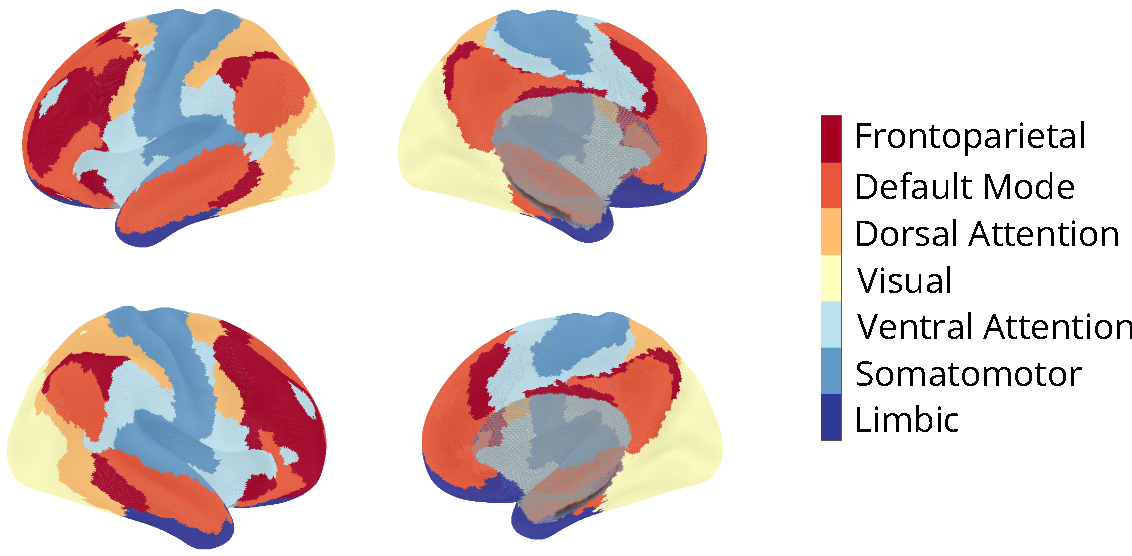
\includegraphics[width=0.5\textwidth]{docs/wnar/toc.pdf}
\end{frame}

% section %
\section{1. Introduction}

% slide %
\begin{frame}{\textcolor{gray}{Estimating fMRI} Timescale Maps}
    \centering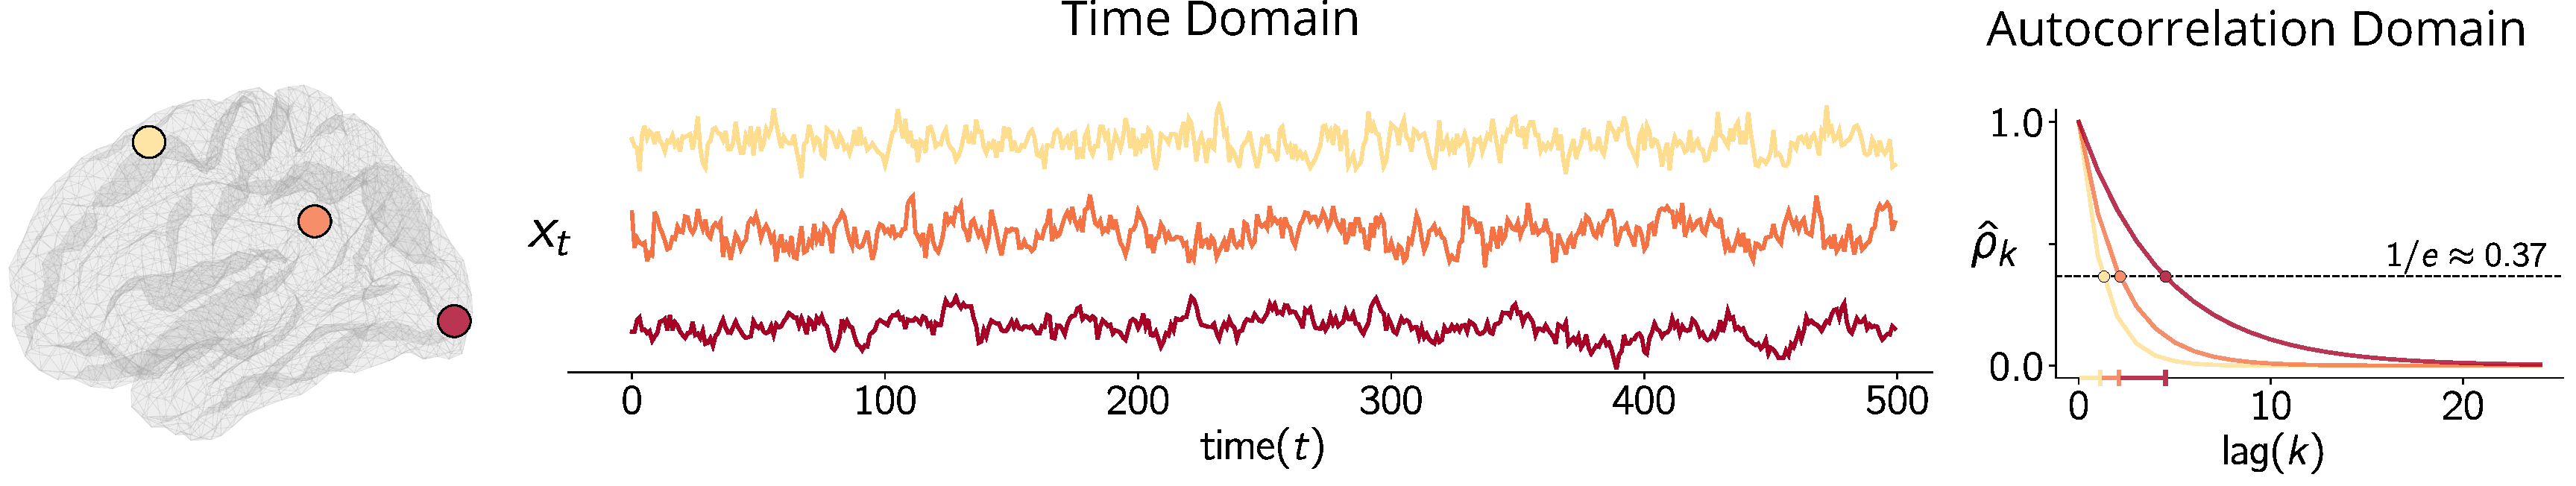
\includegraphics[width=0.95\textwidth]{docs/wnar/timescale.pdf}
    \vfill
    \begin{columns}
    \column{0.8\textwidth}
        \begin{itemize}
        \item neural time series exhibit time-lagged correlations that decay, reflecting how brain regions integrate information over time
        \item timescale parameters quantify the rate of this decay
        \item timescale maps reveal a hierarchical organization across the cortex: fast autocorrelation decay in sensory areas, slow in associative areas
    \end{itemize}
    \column{0.2\textwidth}
    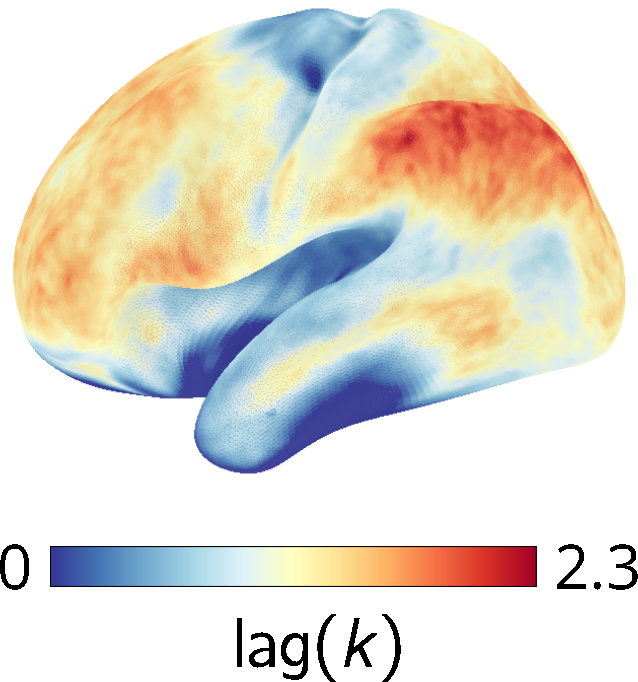
\includegraphics[width=0.85\textwidth]{docs/wnar/timescale-brain.pdf}
    \end{columns}
\end{frame}

% slide %
\begin{frame}{\textcolor{gray}{Estimating} fMRI \textcolor{gray}{Timescale Maps}}
     \centering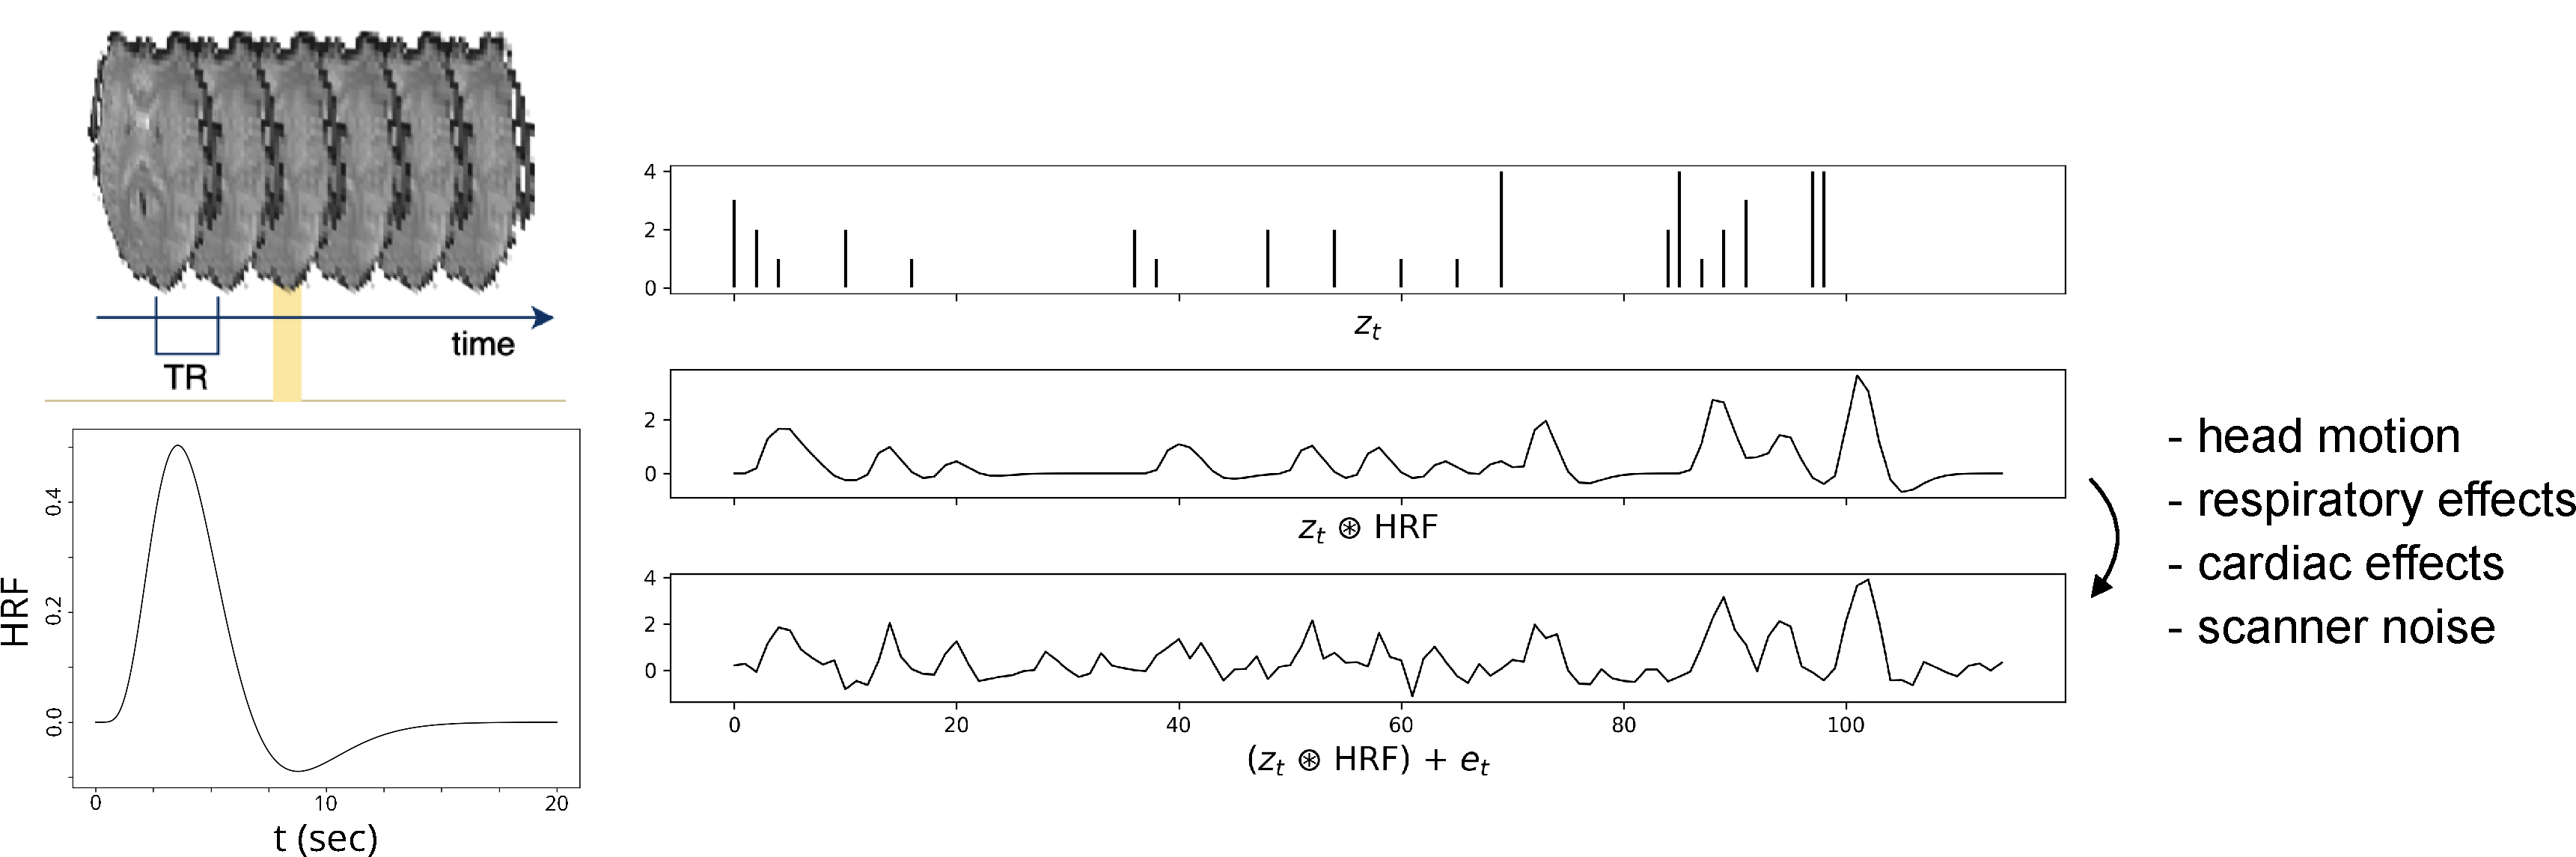
\includegraphics[width=0.95\textwidth]{docs/wnar/fmri.pdf}
     \vfill
     \begin{itemize}
         \item functional magnetic resonance imaging (fMRI), resting-state fMRI (rfMRI)
         \item rfMRI provides whole-brain noninvasive recording of spontaneous brain activity 
         \item reflects hemodynamic changes of the underlying electrical activity of neurons
     \end{itemize}
\end{frame}

% slide %
\begin{frame}{\textcolor{gray}{Estimating} fMRI Timescale Maps}
    \vspace{5mm}
    \centering\includegraphics[width=1\textwidth]{docs/wnar/maps.pdf}
\end{frame}

% slide %
\begin{frame}{Estimating \textcolor{gray}{fMRI Timescale Maps}}

Existing Methods:
\begin{itemize}
    \item time-domain linear model (6/25 papers)
    \item autocorrelation-domain nonlinear model (18/25 papers)
    \item \text{[}\textcolor{gray}{frequency-domain nonlinear model (3/25 papers)}\text{]}
\end{itemize}

\vfill
Limitations of Existing Methods:
\begin{itemize}
    \item assumption of exponentially decaying autocorrelation, which may not hold
    \item point estimates without standard errors, limiting statistical inference
\end{itemize}

\vfill
Paper Contributions:
\begin{itemize}
    \item generalize assumptions to include all stationary and mixing processes
    \item introduce standard errors that account for misspecification
    \item show statistical properties (consistency and asymptotic normality) of time- and autocorrelation-domain methods
    \item show parameter recovery in realistic simulations
    \item apply methods to rfMRI from the Human Connectome Project (HCP)
\end{itemize}

\end{frame}


% section %
\section{2. Methods}

% slide %
\begin{frame}{Assumptions}
Let $\{X_t, t\in \mathbb{Z}\}$ be a discrete-time stochastic process that is \textbf{stationary} and \textbf{strong mixing}, and $x_t = \{x_1, x_2, ..., x_T\}$ be an observed sample of $X_t$. Assume $X_t$ and $x_t$ have mean zero.\\
\vfill
Stationarity Implies:
\begin{align}
    \gamma_k &= \text{cov}[X_t, X_{t-k}] = \mathbb{E}[X_t X_{t-k}]\\
    \rho_k &= \text{corr}[X_t, X_{t-k}] = \gamma_0^{-1}\gamma_k\label{acf}
\end{align}

Mixing Implies:
\begin{itemize}
    \item ergodicity, ensuring consistent estimation by the ergodic theorem
    \item autocorrelations \eqref{acf} decay sufficiently fast for the central limit theorem for correlated observations to apply
\end{itemize}
\vfill
\citet{hansen_econometrics_2022, white_nonlinear_1984, newey_simple_1987}\\
\end{frame}

% slide %
\begin{frame}{Time-Domain Linear Model}
\vfill
Autoregressive Model (AR1) Definition:
\begin{align}
    X_t = \phi X_{t-1} + e_t
\end{align}

\onslide<2->
Squared Error Minimization:
\begin{align}
    S(\phi) = \mathbb{E}[(X_t - \phi X_{t-1})^2],\quad \phi^* = \underset{\phi}{\text{argmin}} \; S(\phi)
\end{align}

\onslide<3->
Timescale Definition:
\begin{align}
    \phi^* &= (\mathbb{E}[X_{t-1}^2])^{-1}(\mathbb{E}[X_t X_{t-1}])\\
    \tau^* &= g(\phi^*) = -\frac{1}{\text{log}(|\phi^*|)}
\end{align}

\onslide<4->
Linear Least Squares (LLS) Estimation:
\begin{align}
    \hat\phi^*_{\scriptscriptstyle\text{LLS}} &= \left(\sum_{t=2}^T x_{t-1}^2\right)^{-1} \left(\sum_{t=2}^T x_t x_{t-1}\right)\\
    \hat\tau^*_{\scriptscriptstyle\text{LLS}} &= g(\hat\phi_{\scriptscriptstyle\text{LLS}}) = -\frac{1}{\text{log}(|\hat\phi_{\scriptscriptstyle\text{LLS}}|)}
\end{align}

\end{frame}


% slide %
\begin{frame}{Autocorrelation-Domain Nonlinear Model}
\vfill
Exponential Decay Model Definition:
\begin{align}\label{eq:nlm}
    \rho_k = \phi^k + e_k, \; \text{for}\; k \in \{0, 1, \ldots, K\}
\end{align}

\onslide<2->
Squared Error Minimization:
\begin{align}\label{eq:nlm_loss}
    S(\phi) = \mathbb{E}[(\rho_k - \phi^k)^2], \quad \phi^* = \underset{\phi}{\text{argmin}} \; S(\phi)
\end{align}

\onslide<3->
Timescale Definition:
\begin{align}
    \tau^* &= g(\phi^*) = -\frac{1}{\text{log}(|\phi^*|)} \label{eq:nlm-tau}
\end{align}

\onslide<4->
Nonlinear Least Squares (NLS) Estimation:
\begin{align}
    \hat \phi^*_{\scriptscriptstyle\text{NLS}} &= \underset{\phi}{\text{argmin}} \; \widehat{S}(\phi) \label{eq:nls_phi_}\\
    \hat \tau^*_{\scriptscriptstyle\text{NLS}} &= g(\hat \phi^*_{\scriptscriptstyle\text{NLS}}) = -\frac{1}{\text{log}(|\hat\phi_{\scriptscriptstyle\text{NLS}}|)}
\end{align}

\end{frame}

% slide %
\begin{frame}{Standard Error Estimation}

Time-Domain Method:
\begin{align}\label{eq:stderr-time-domain_}
\widehat{\text{se}}_{\text{NW}}(\hat\phi^*_{\scriptscriptstyle\text{LLS}}) = \sqrt{\hat q^{-1}\;\hat\omega\; \hat q^{-1}}, \quad
\widehat{\text{se}}_{\text{NW}}(\hat\tau^*_{\scriptscriptstyle\text{LLS}}) \approx \widehat{\text{se}}_{\text{NW}}(\hat\phi^*_{\scriptscriptstyle\text{LLS}}) \cdot \frac{d}{d\phi} g(\hat\phi^*_{\scriptscriptstyle\text{LLS}})
\end{align}

\begin{align}\label{eq:lls_q_omega_}
    \hat q = \frac{1}{T} \sum_{t=2}^T x_{t-1}^2, \quad
    \hat \omega = \sum_{\ell=-M}^M \left(1 - \frac{|\ell|}{M+1}\right) \; \frac{1}{T} \sum_{1\le t - \ell \le T} (x_{t-1} \cdot \hat e_t)(x_{t-1-\ell} \cdot \hat e_{t-\ell})
\end{align}

\onslide<2->
Autocorrelation-Domain Method:
\begin{align}\label{eq:stderr-autocorrelation-domain_}
\widehat{\text{se}}_{\text{NW}}(\hat\phi^*_{\scriptscriptstyle\text{NLS}}) = \sqrt{\hat q^{-1}\;\hat\omega\; \hat q^{-1}}, \quad
\widehat{\text{se}}_{\text{NW}}(\hat\tau^*_{\scriptscriptstyle\text{NLS}}) \approx \widehat{\text{se}}_{\text{NW}}(\hat\phi^*_{\scriptscriptstyle\text{NLS}}) \cdot \frac{d}{d\phi} g(\hat\phi^*_{\scriptscriptstyle\text{NLS}})
\end{align}

\begin{align}
    \hat q &= \frac{1}{K} \sum_{k=0}^K (\hat m_{\phi,k})^2 = \frac{1}{K} \sum_{k=0}^K (k \hat\phi_{\scriptscriptstyle\text{NLS}}^{*k-1})^2, \quad
    \hat \omega = \sum_{\ell=-M}^M \left(1 - \frac{|\ell|}{M+1}\right) \; \frac{1}{K} \sum_{1 \le k - \ell \le K} (\hat m_{\phi, k} \cdot \hat e_k) (\hat m_{\phi, k-\ell} \cdot \hat e_{k-\ell})
\end{align}

\onslide<3->
Autocorrelation/Time-Domain Method, equation \eqref{eq:stderr-time-domain_} except for:
\begin{align}
    \hat e_t = x_t - \hat\phi^*_{\scriptscriptstyle\text{NLS}} \cdot x_{t-1}
\end{align}
\end{frame}


% section %
\section{3. Simulations}

% slide %
\begin{frame}{AR1 Simulations}
\vspace{1.5mm}
$N=10,000$ repeats, $T = 4,800$ timepoints \\ 
$x_t = \phi x_{t-1} + e_t, \; e_t \sim \mathcal{N}(0, 1)$ \quad \textcolor{gray}{$\rho_k = \phi^k + e_k,\; e_k \sim \mathcal{N}(0, 1)$}
\vspace{1.5mm}

\centering
\only<1>{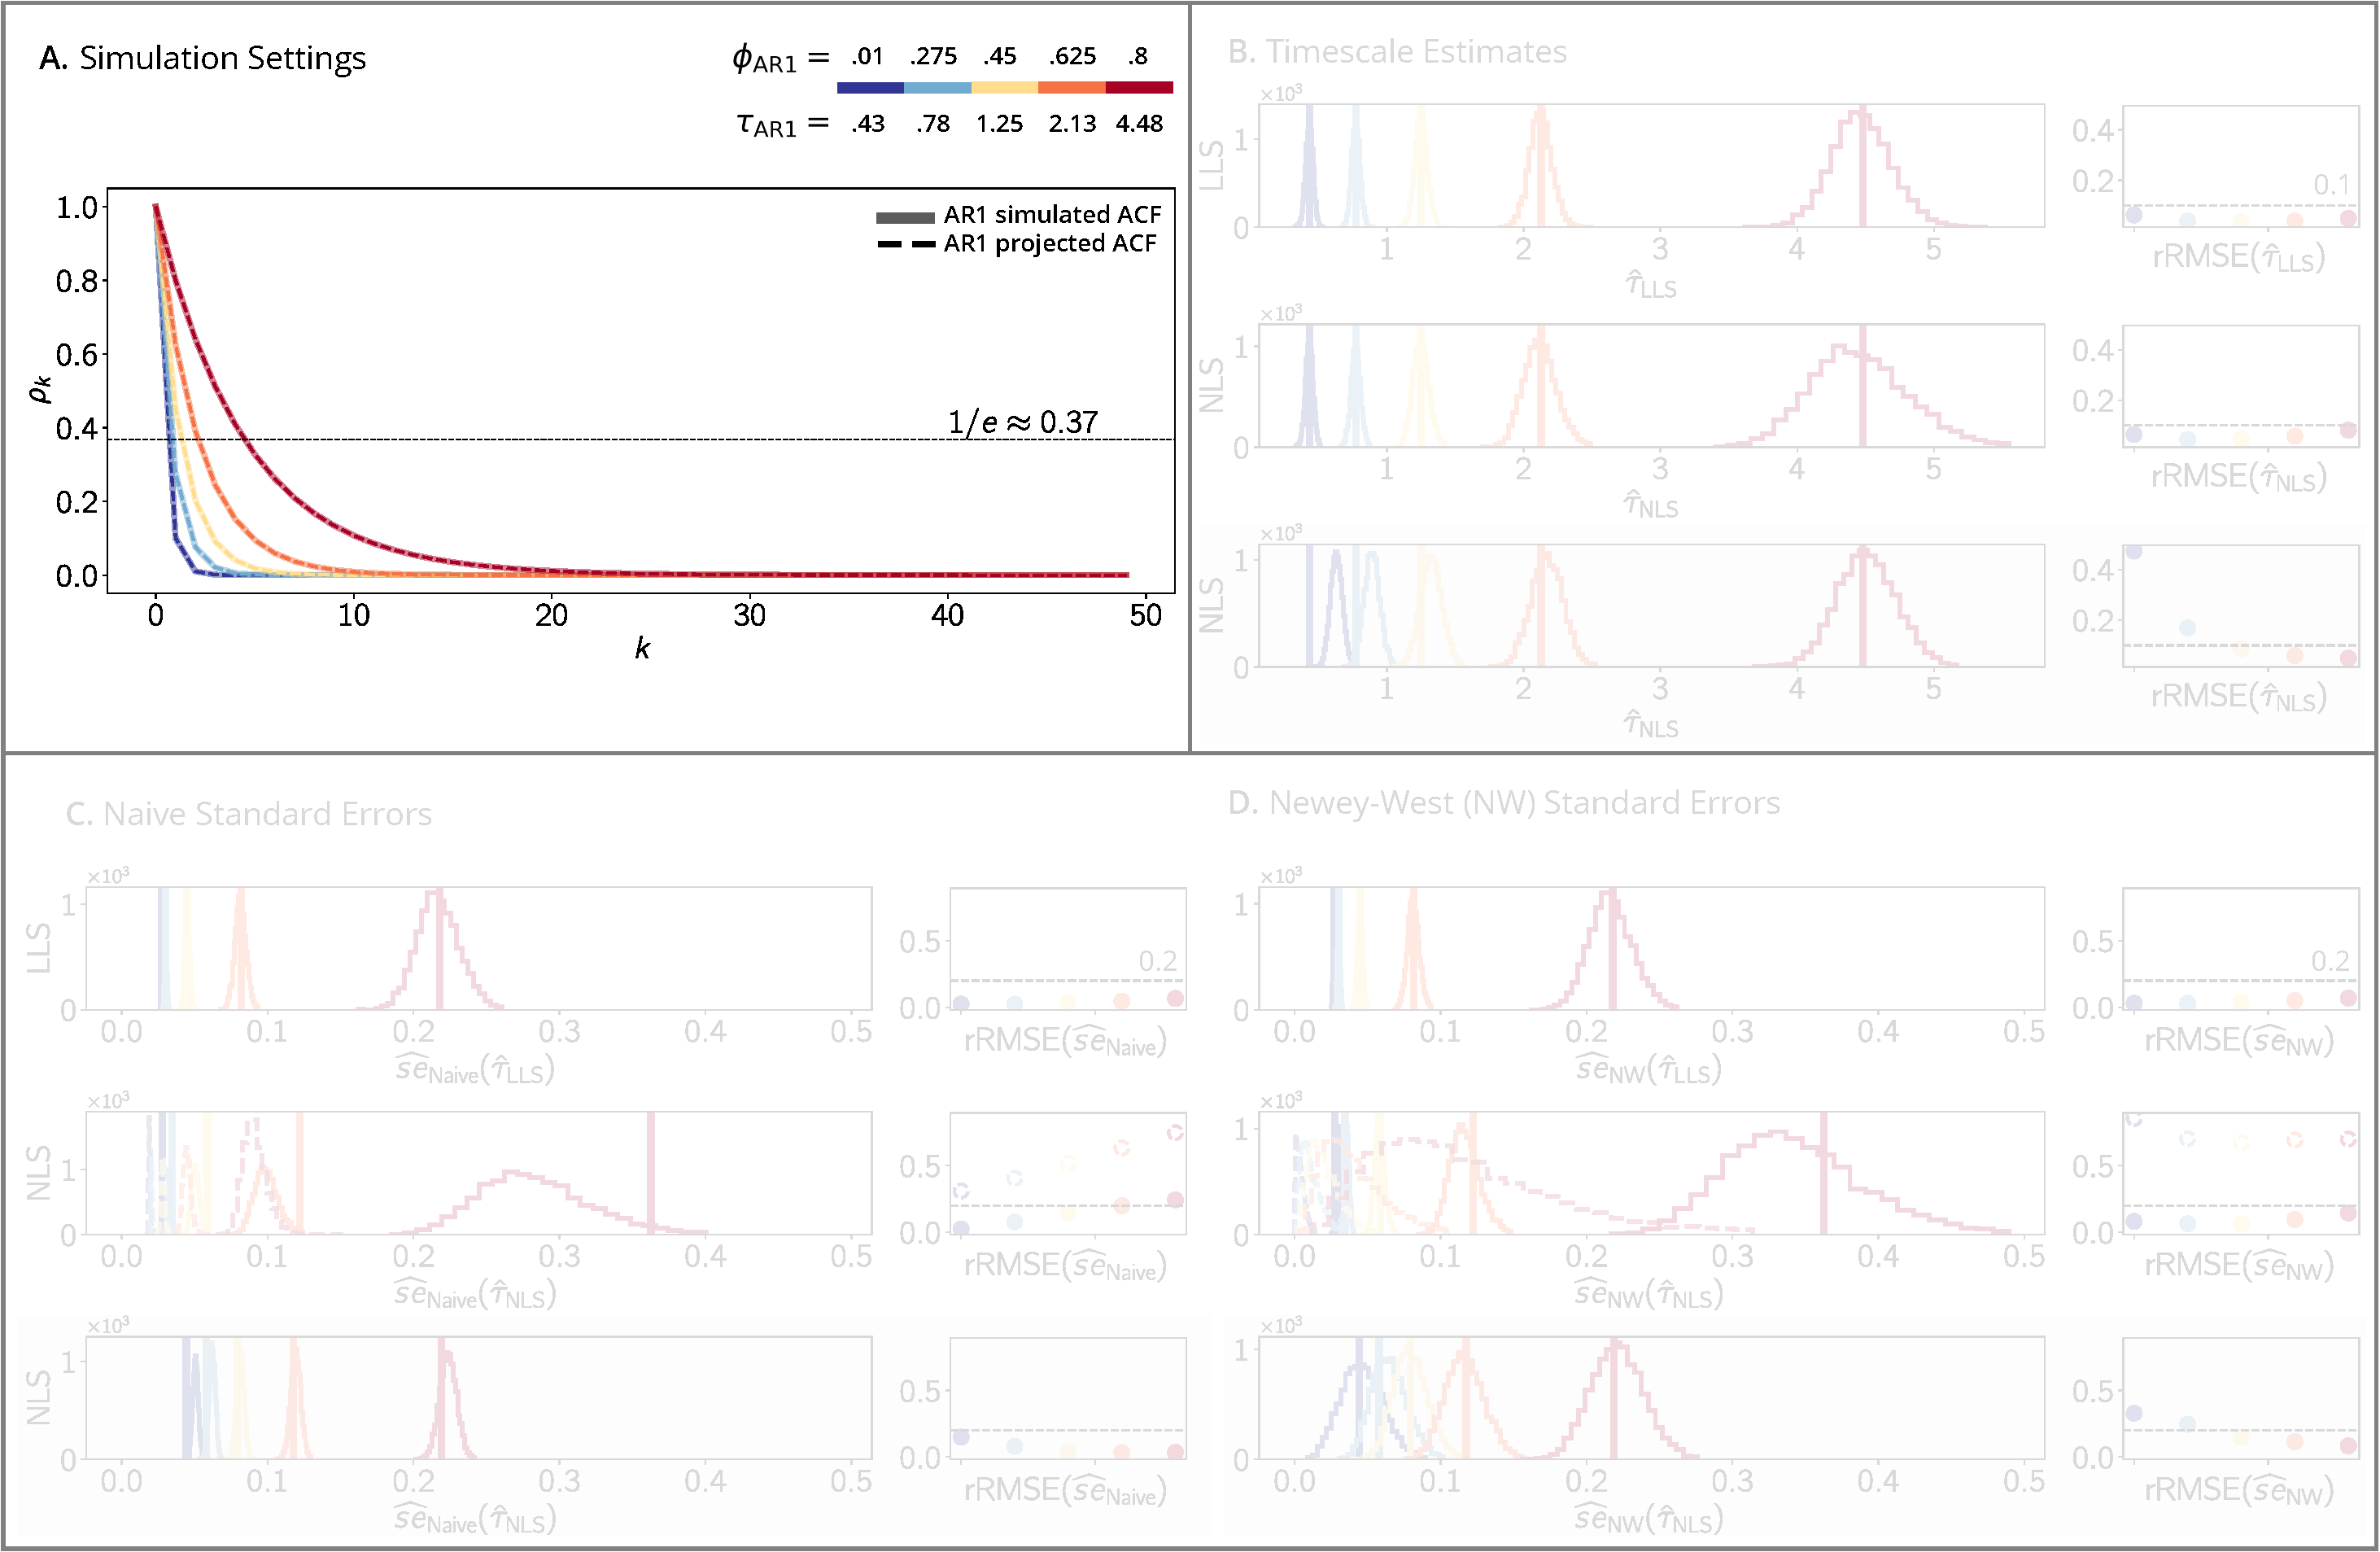
\includegraphics[width=0.85\textwidth]{docs/wnar/ar1-results-1.pdf}}
\only<2>{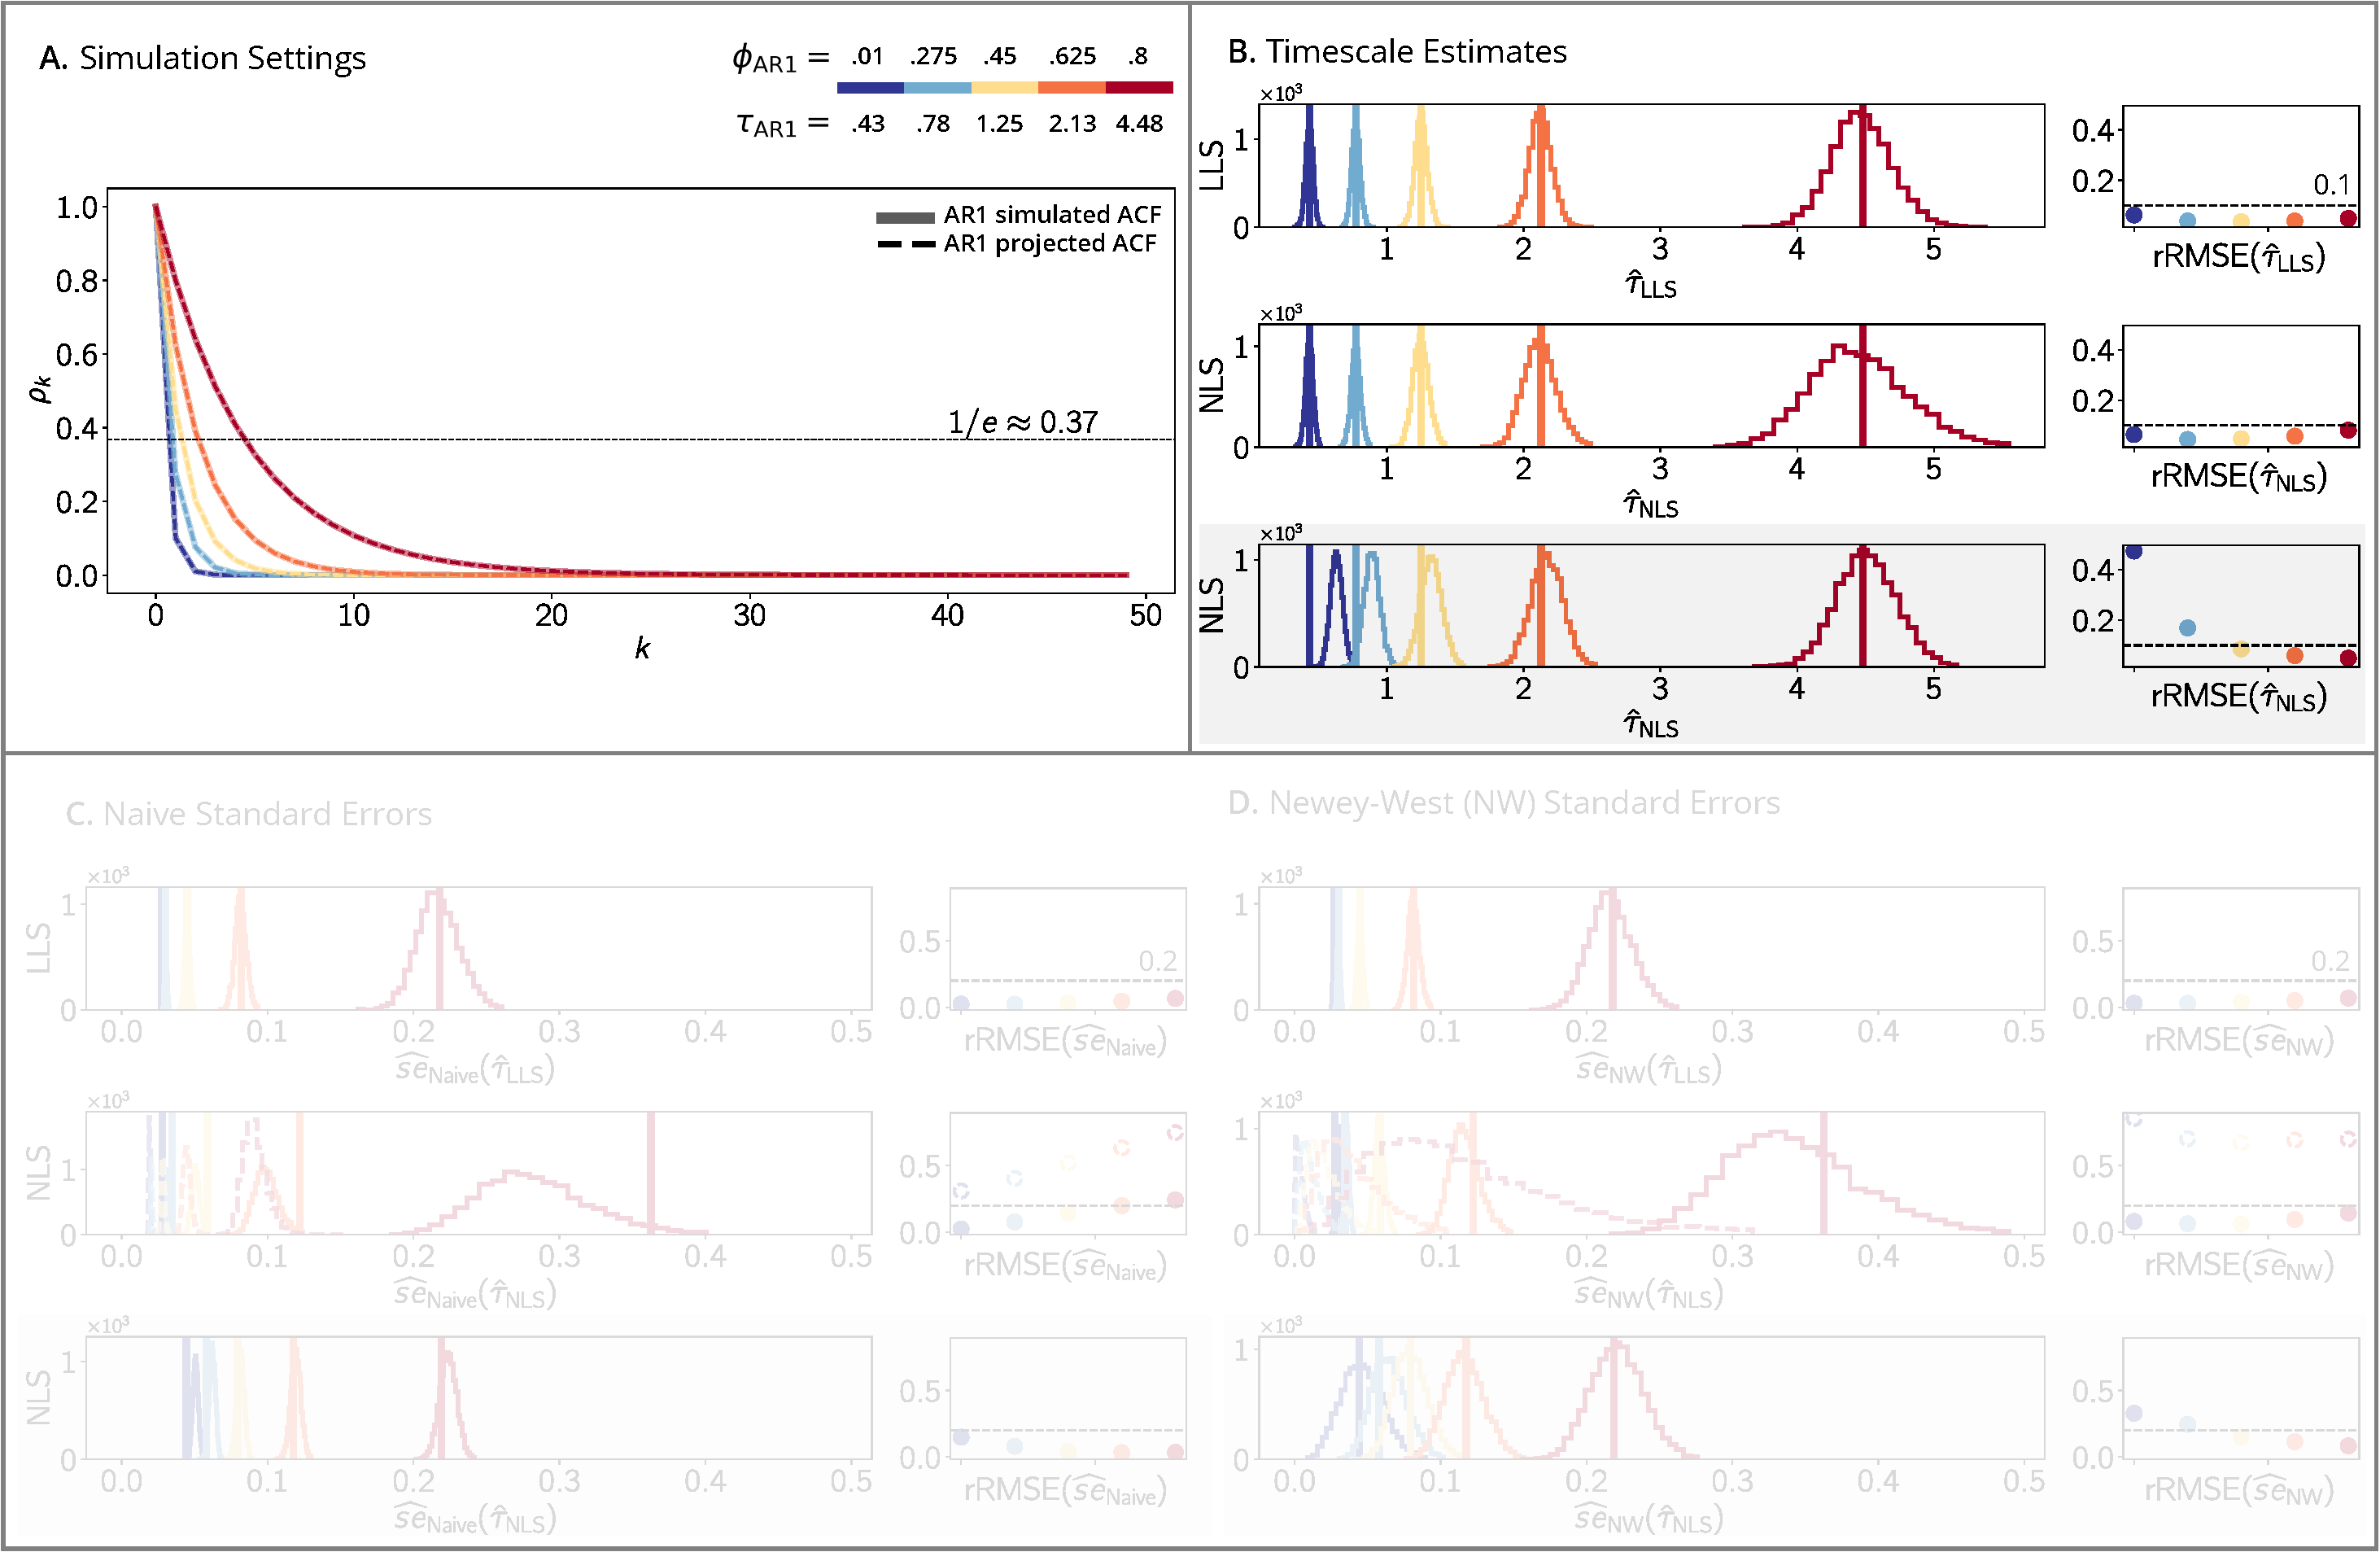
\includegraphics[width=0.85\textwidth]{docs/wnar/ar1-results-2.pdf}}
\only<3>{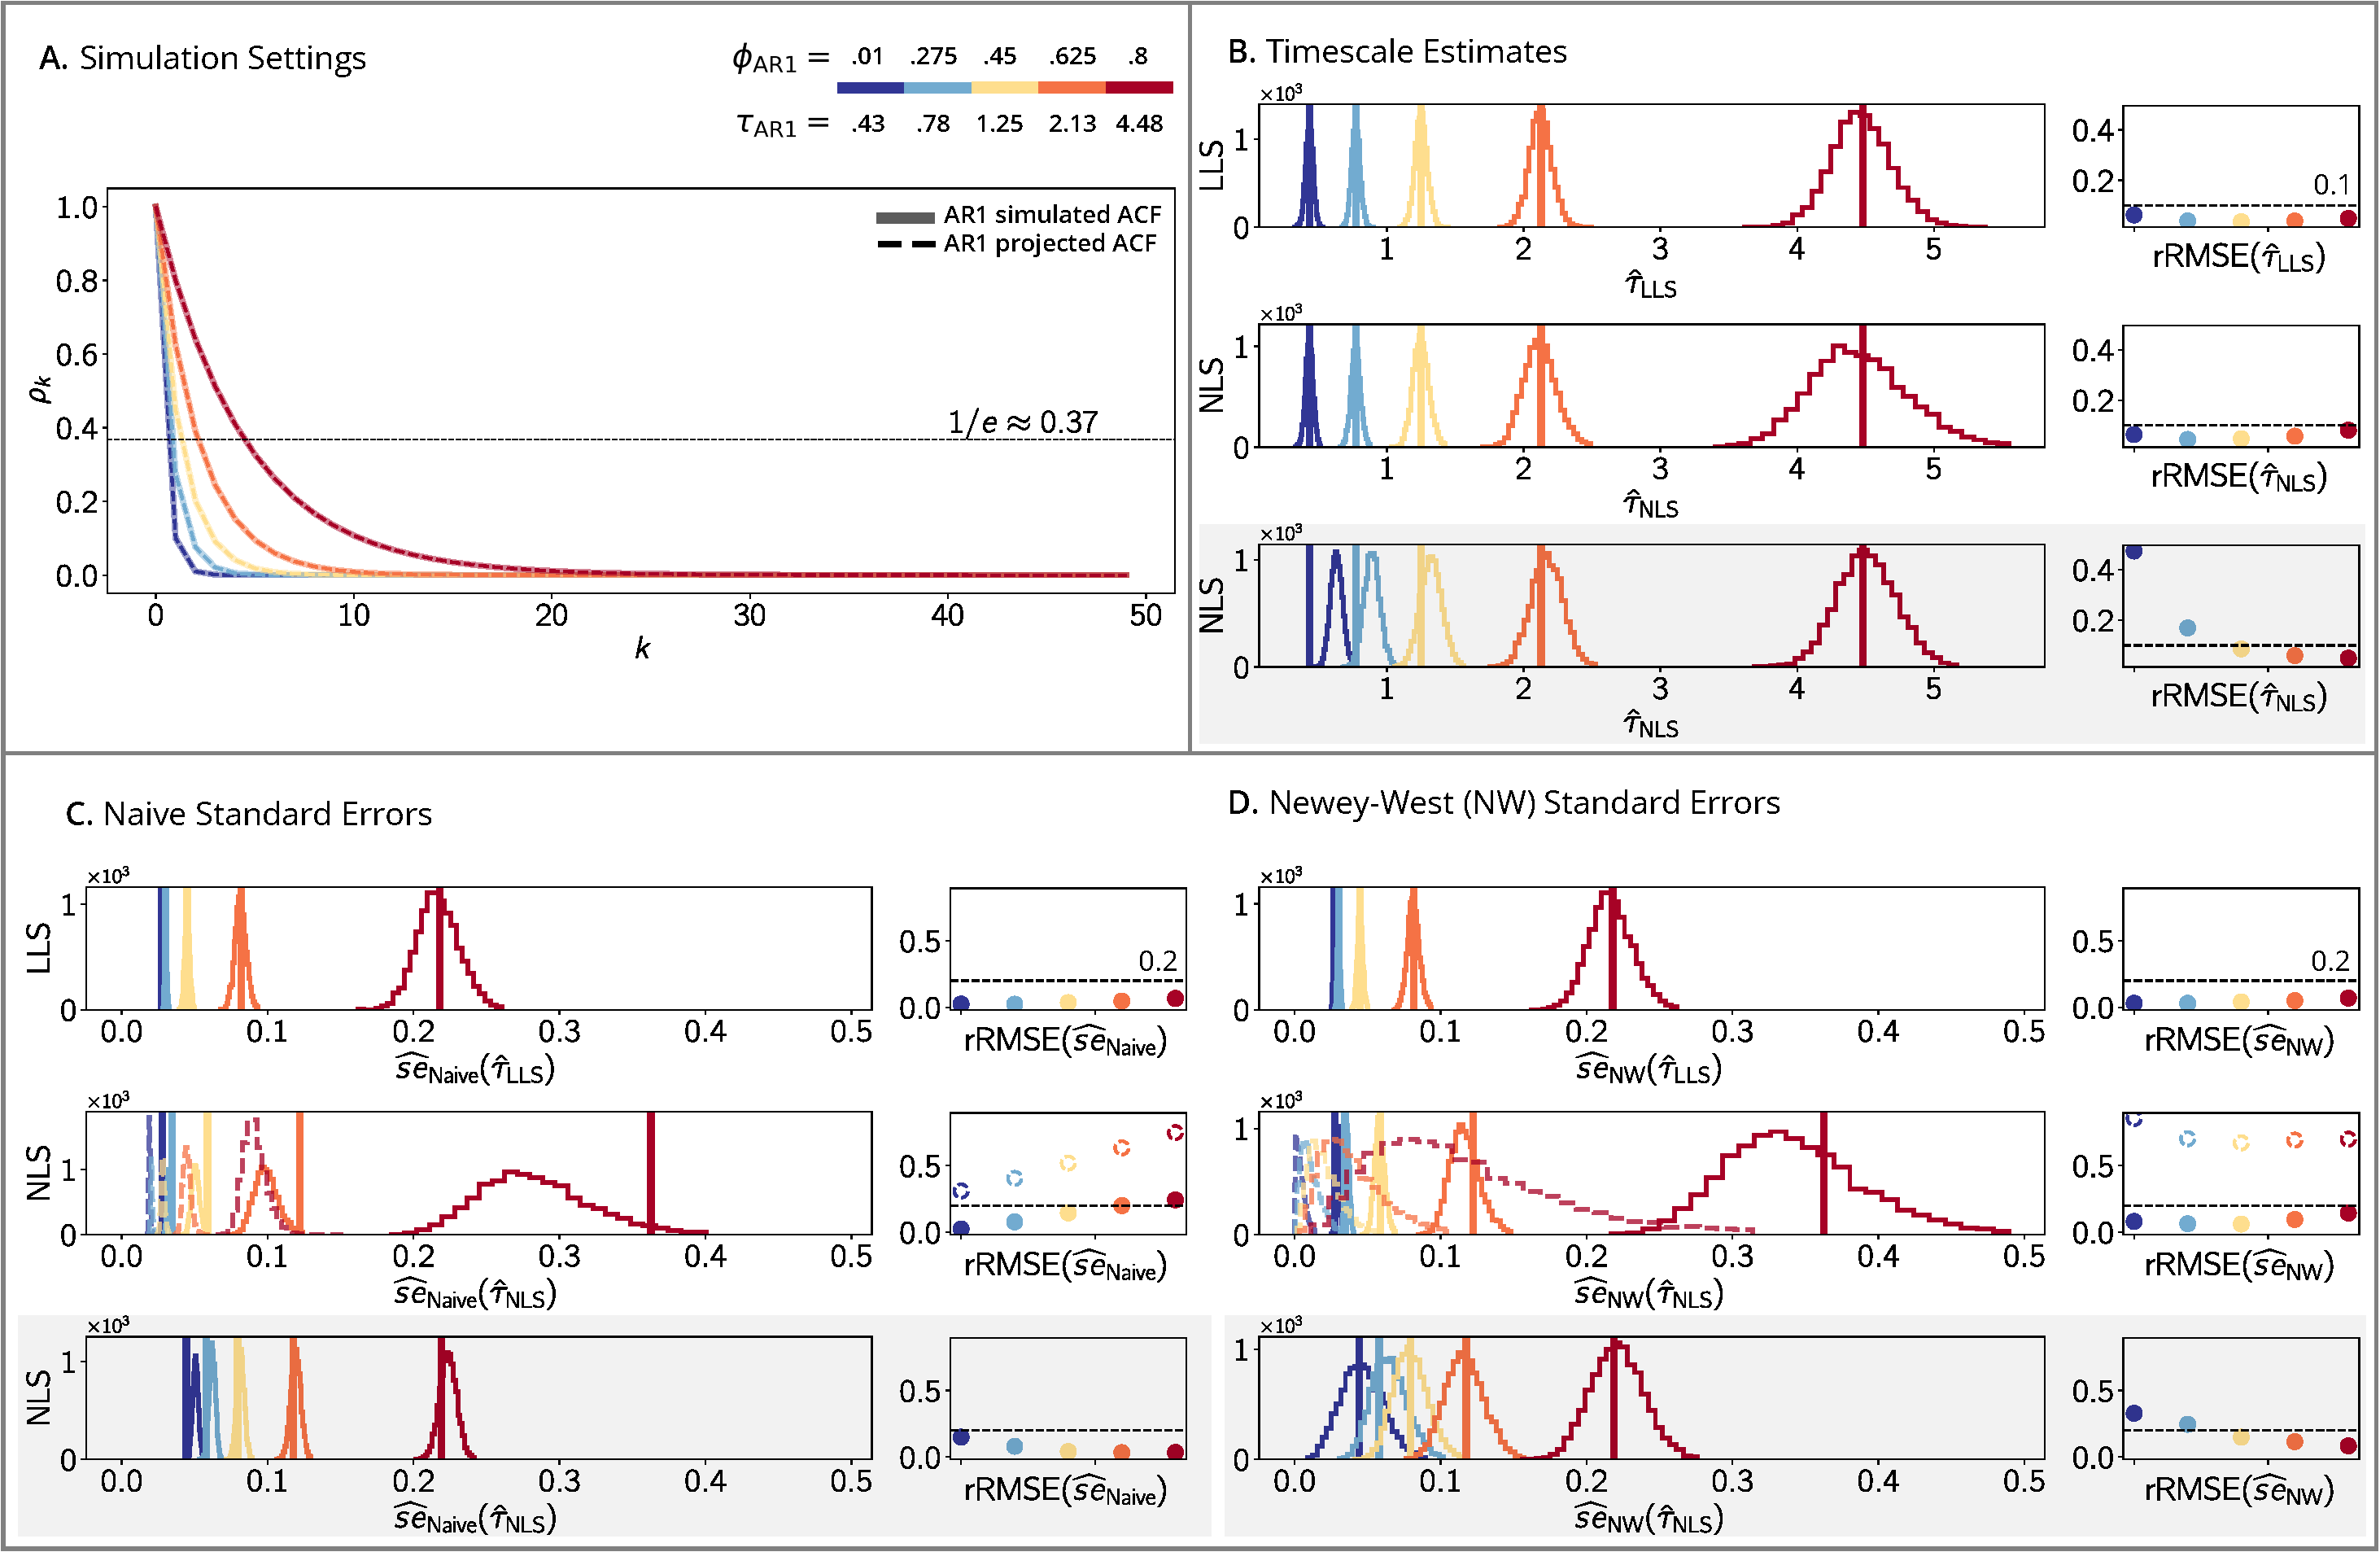
\includegraphics[width=0.85\textwidth]{docs/wnar/ar1-results-3.pdf}}
\end{frame}

% slide %
\begin{frame}{AR2 Simulations}
\vspace{1.5mm}
$N=10,000$ repeats, $T = 4,800$ timepoints \\ 
$x_t = \phi_1 x_{t-1} + \phi_2 x_{t-2} +e_t, \; e_t \sim \mathcal{N}(0, 1)$ \quad \textcolor{gray}{$\rho_k = \phi_1\rho_{k-1} + \phi_2\rho_{k-2} + e_k,\; e_k \sim \mathcal{N}(0, 1)$}
\vspace{1.5mm}

\centering
\only<1>{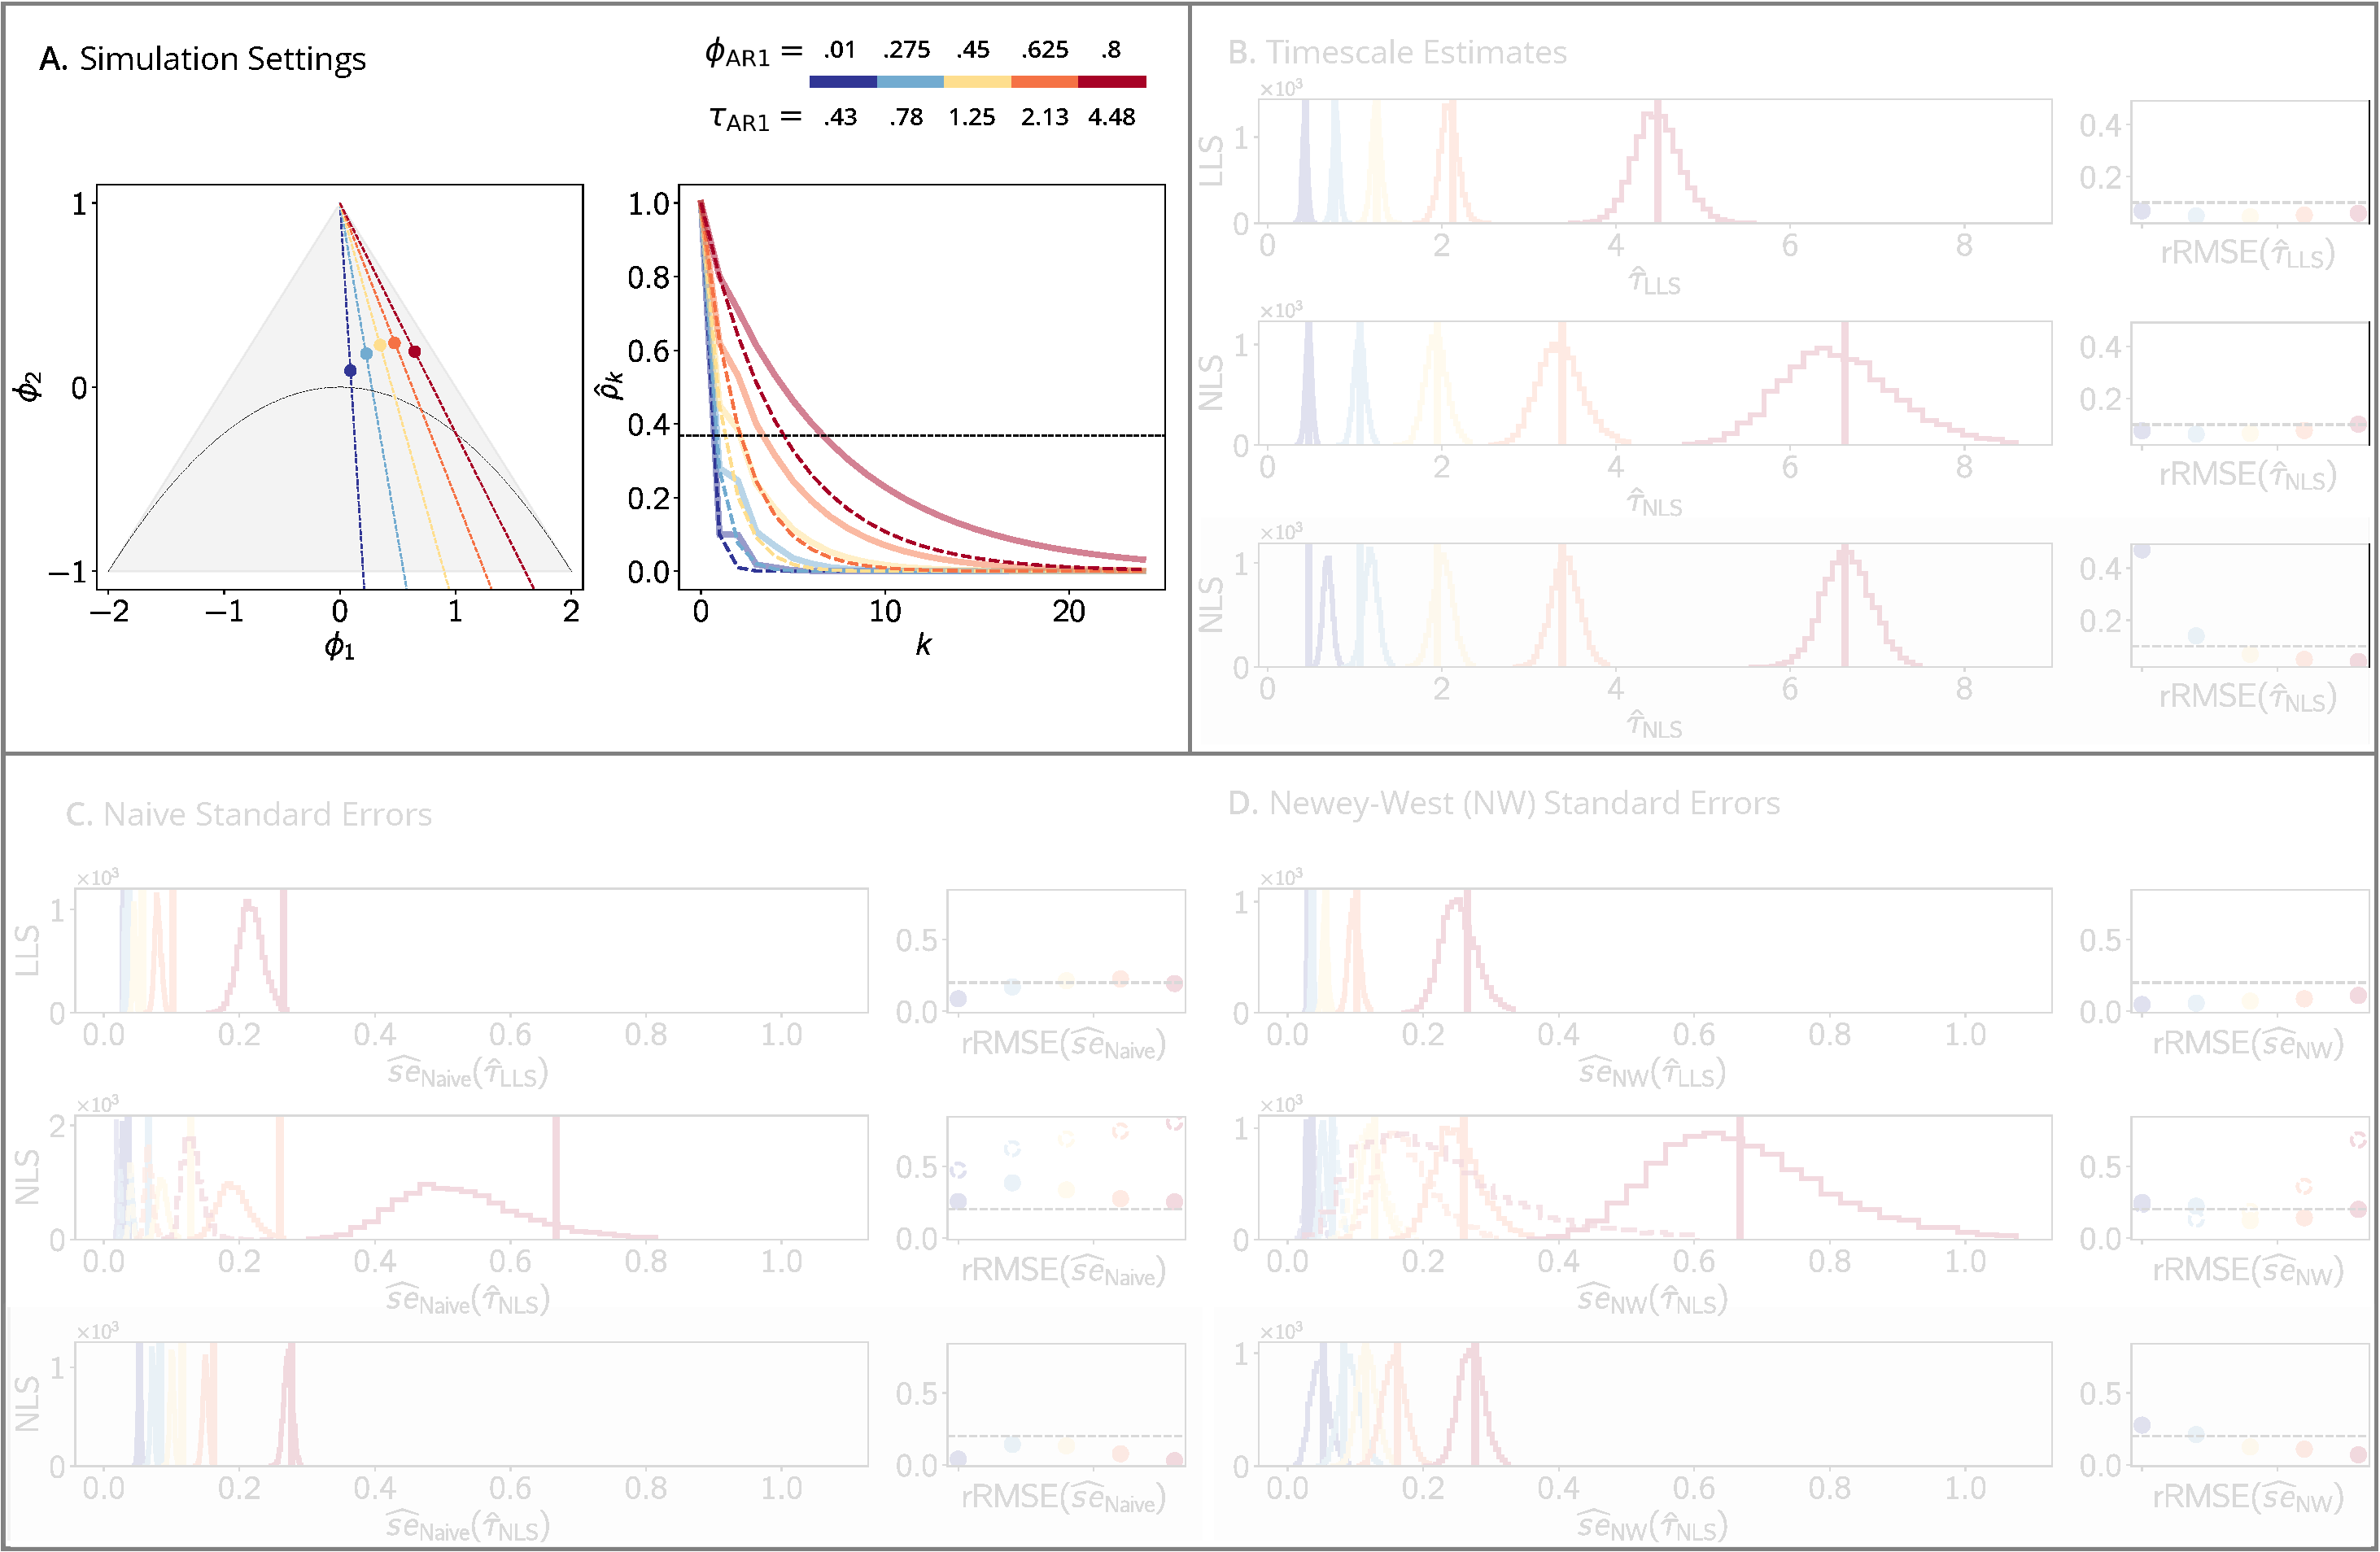
\includegraphics[width=0.85\textwidth]{docs/wnar/ar2-results-1.pdf}}
\only<2>{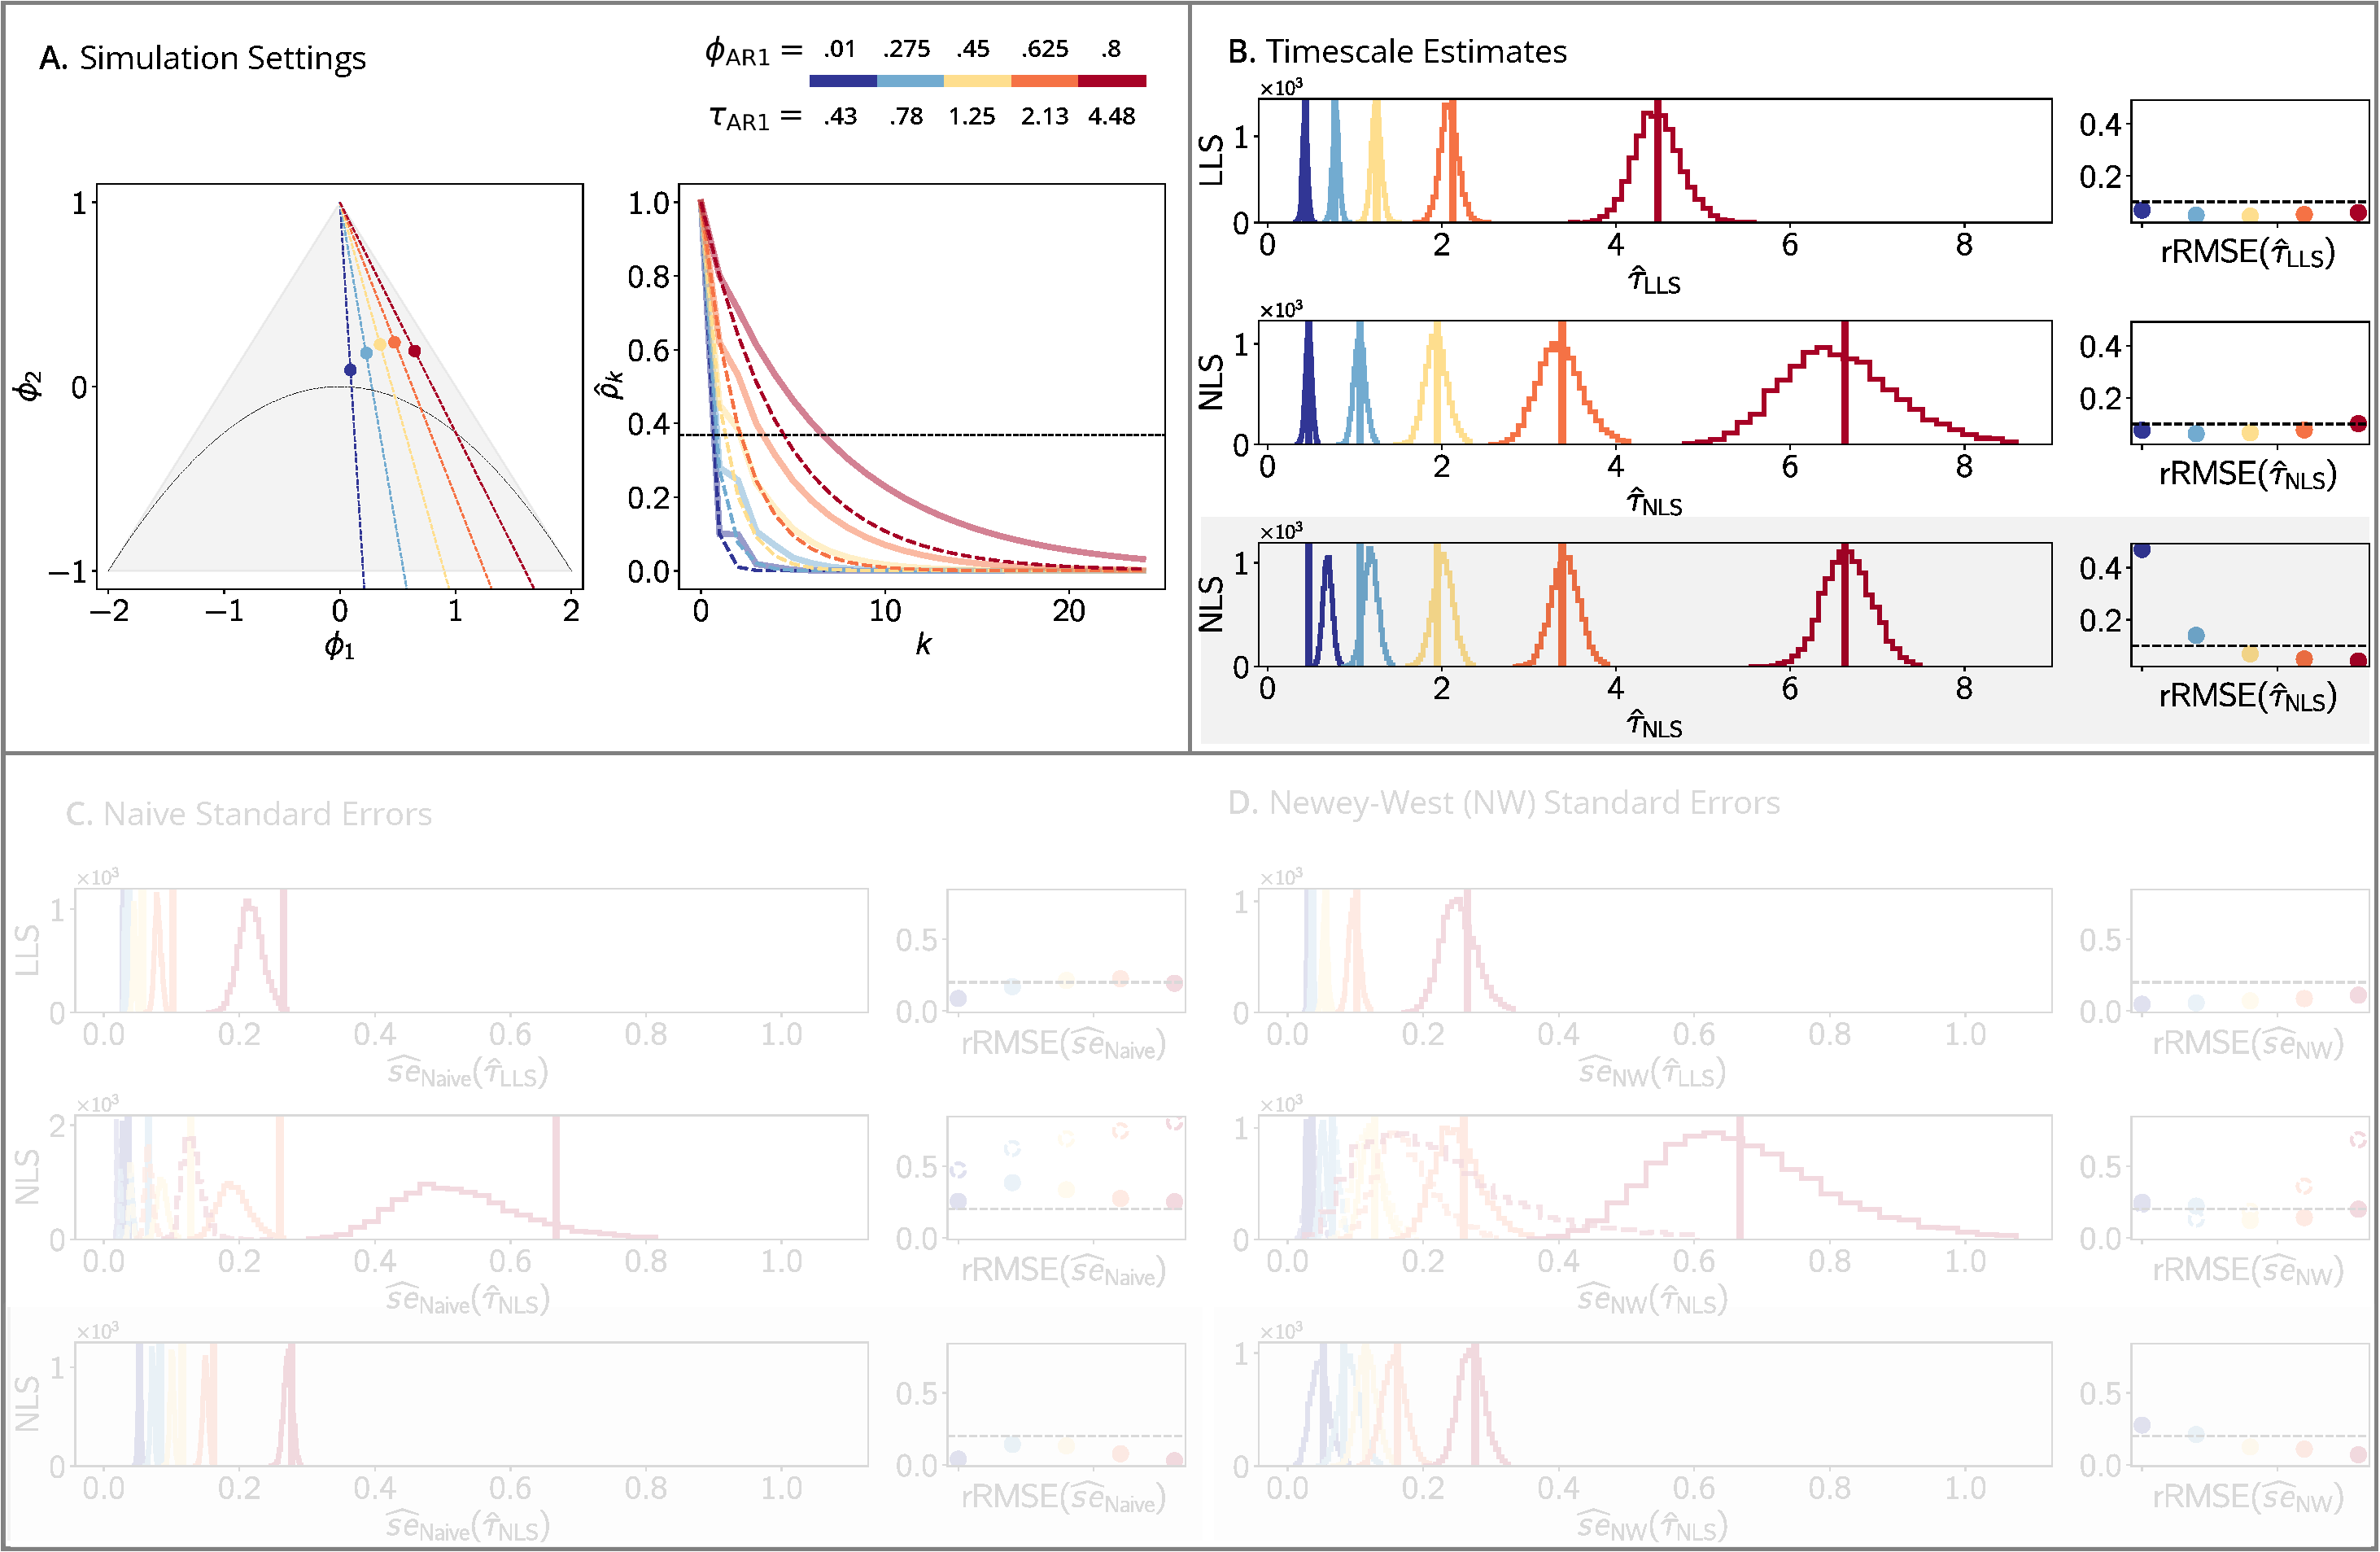
\includegraphics[width=0.85\textwidth]{docs/wnar/ar2-results-2.pdf}}
\only<3>{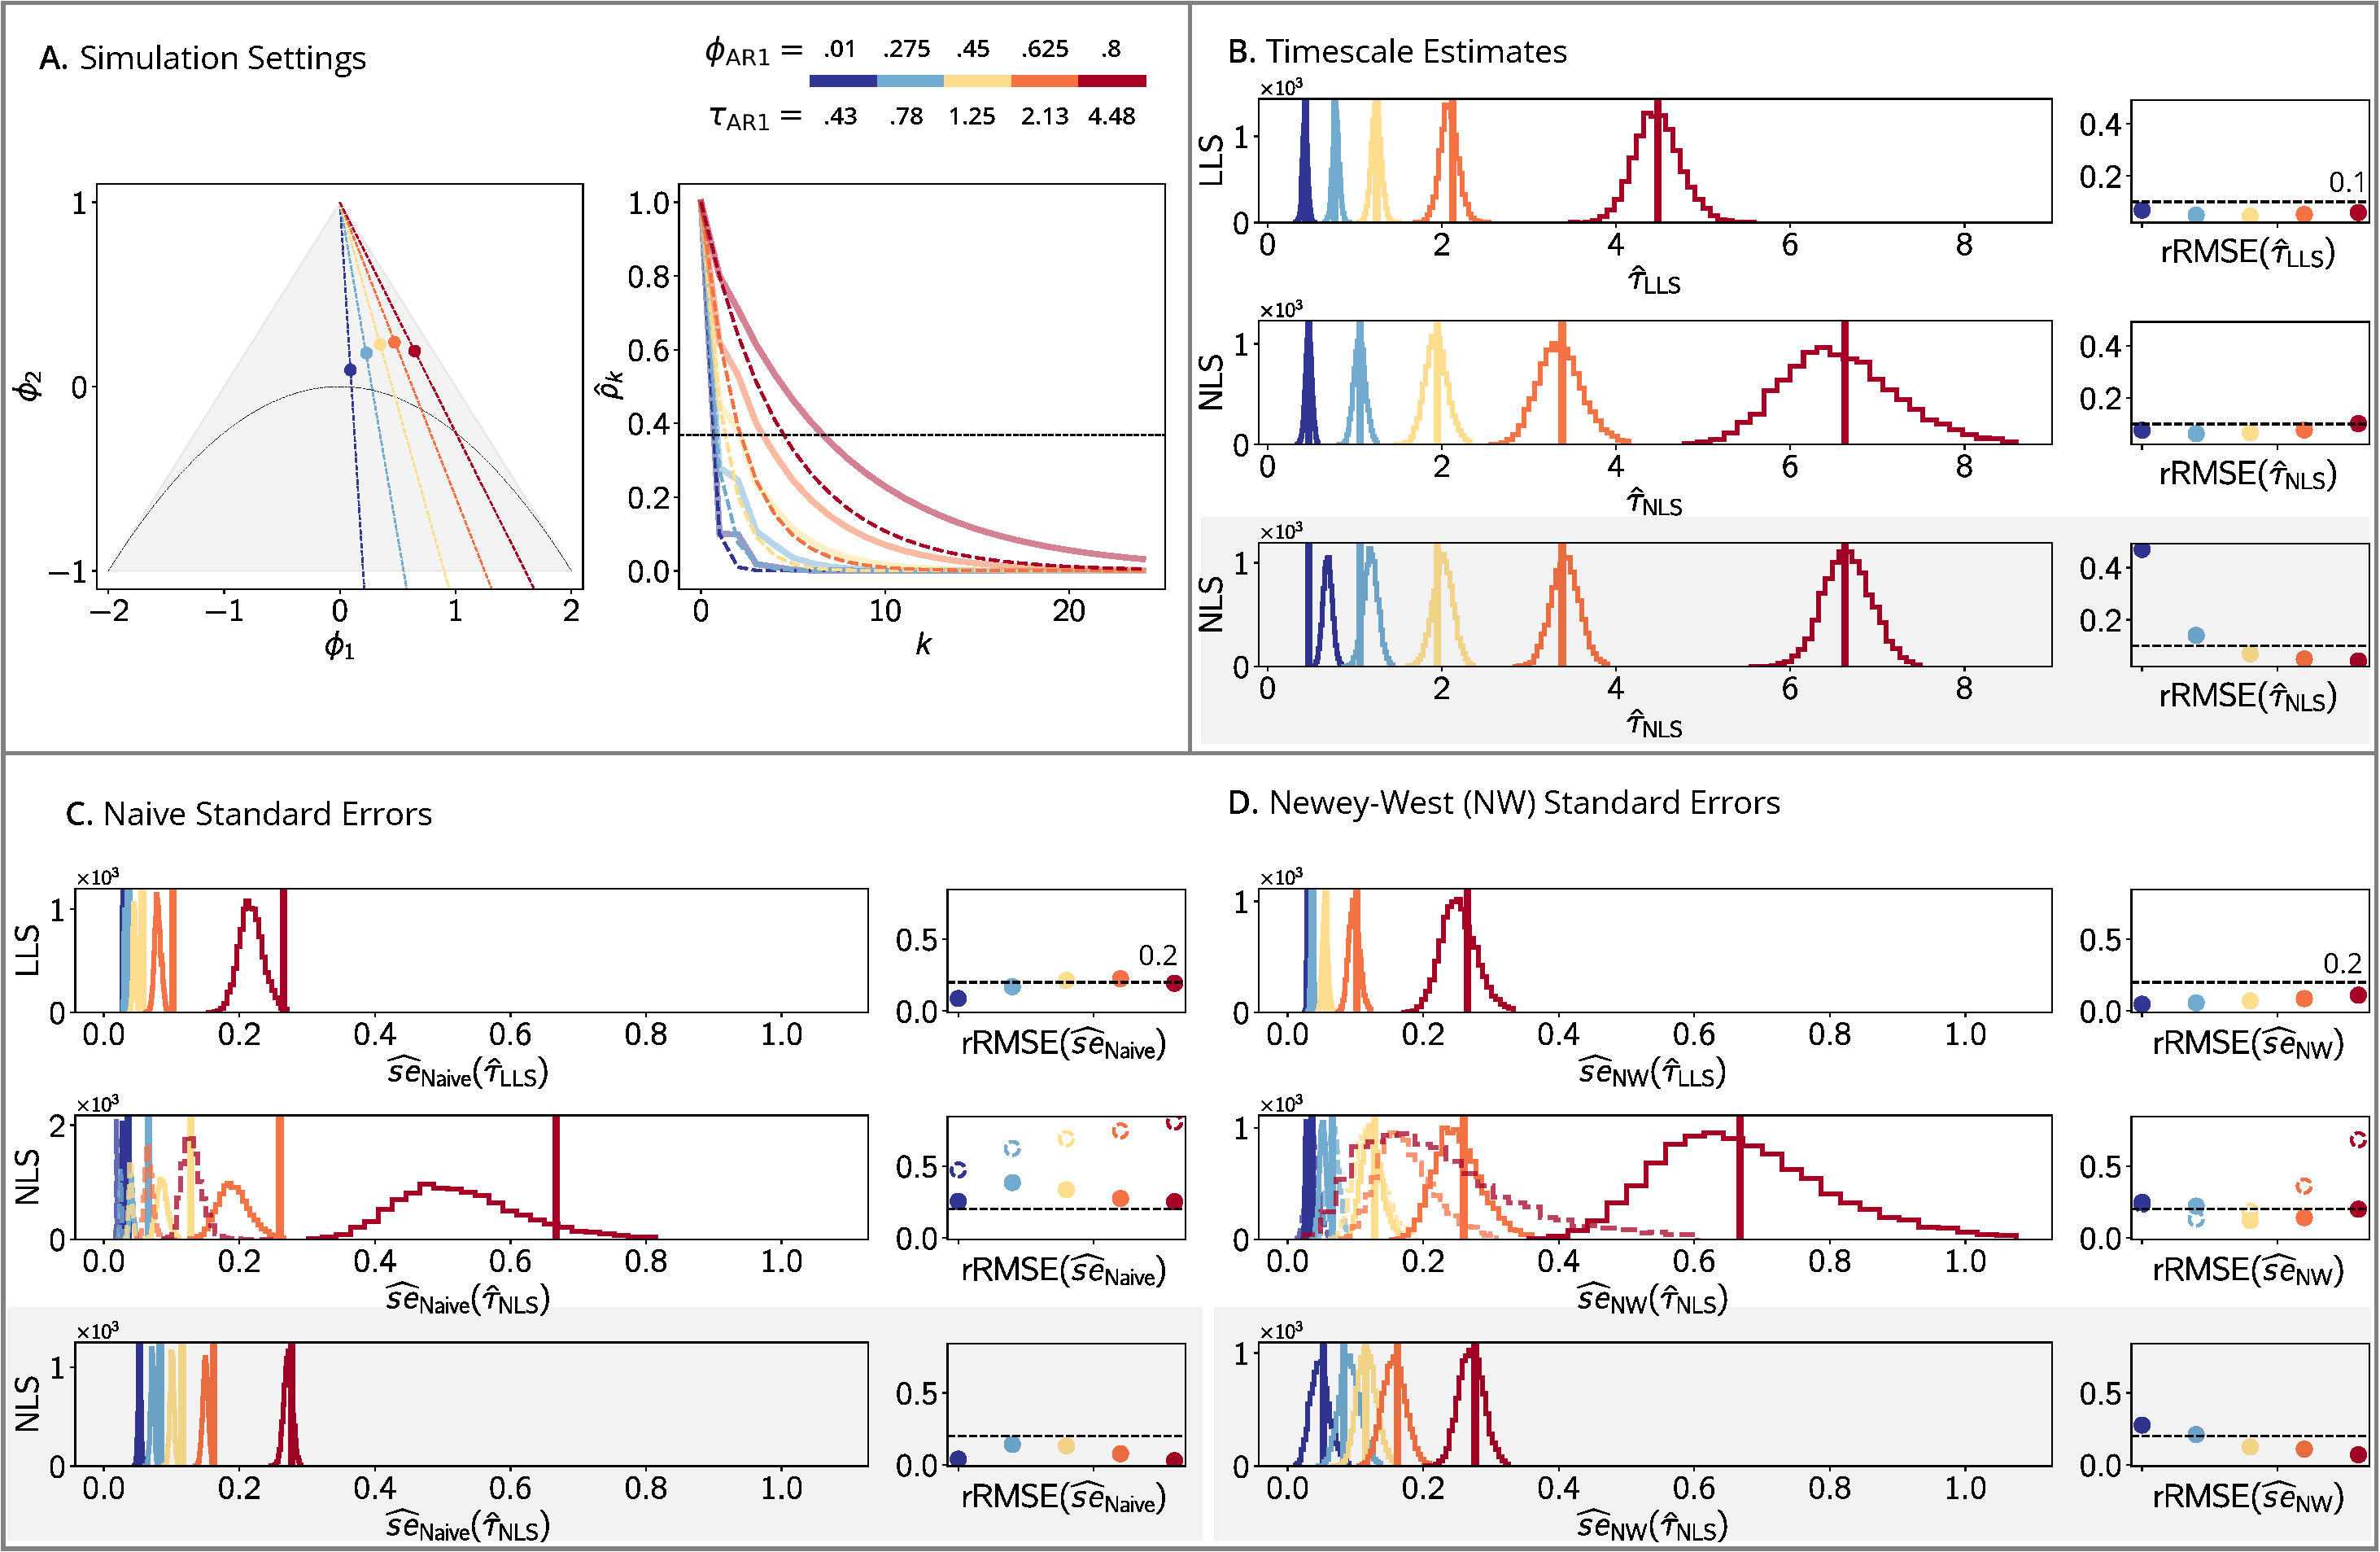
\includegraphics[width=0.85\textwidth]{docs/wnar/ar2-results-3.pdf}}
\end{frame}


% slide %
\begin{frame}{Realistic rfMRI Simulations}
\vspace{1.5mm}
$N=10,000$ repeats, $T = 4,800$ timepoints \\ 
$x_t \sim \mathcal{N}(0, \hat\Sigma)$ \quad \textcolor{gray}{$\rho_k = \hat\rho_k + e_k,\; e_k \sim \mathcal{N}(0, 1)$}
\vspace{1.5mm}

\centering
\only<1>{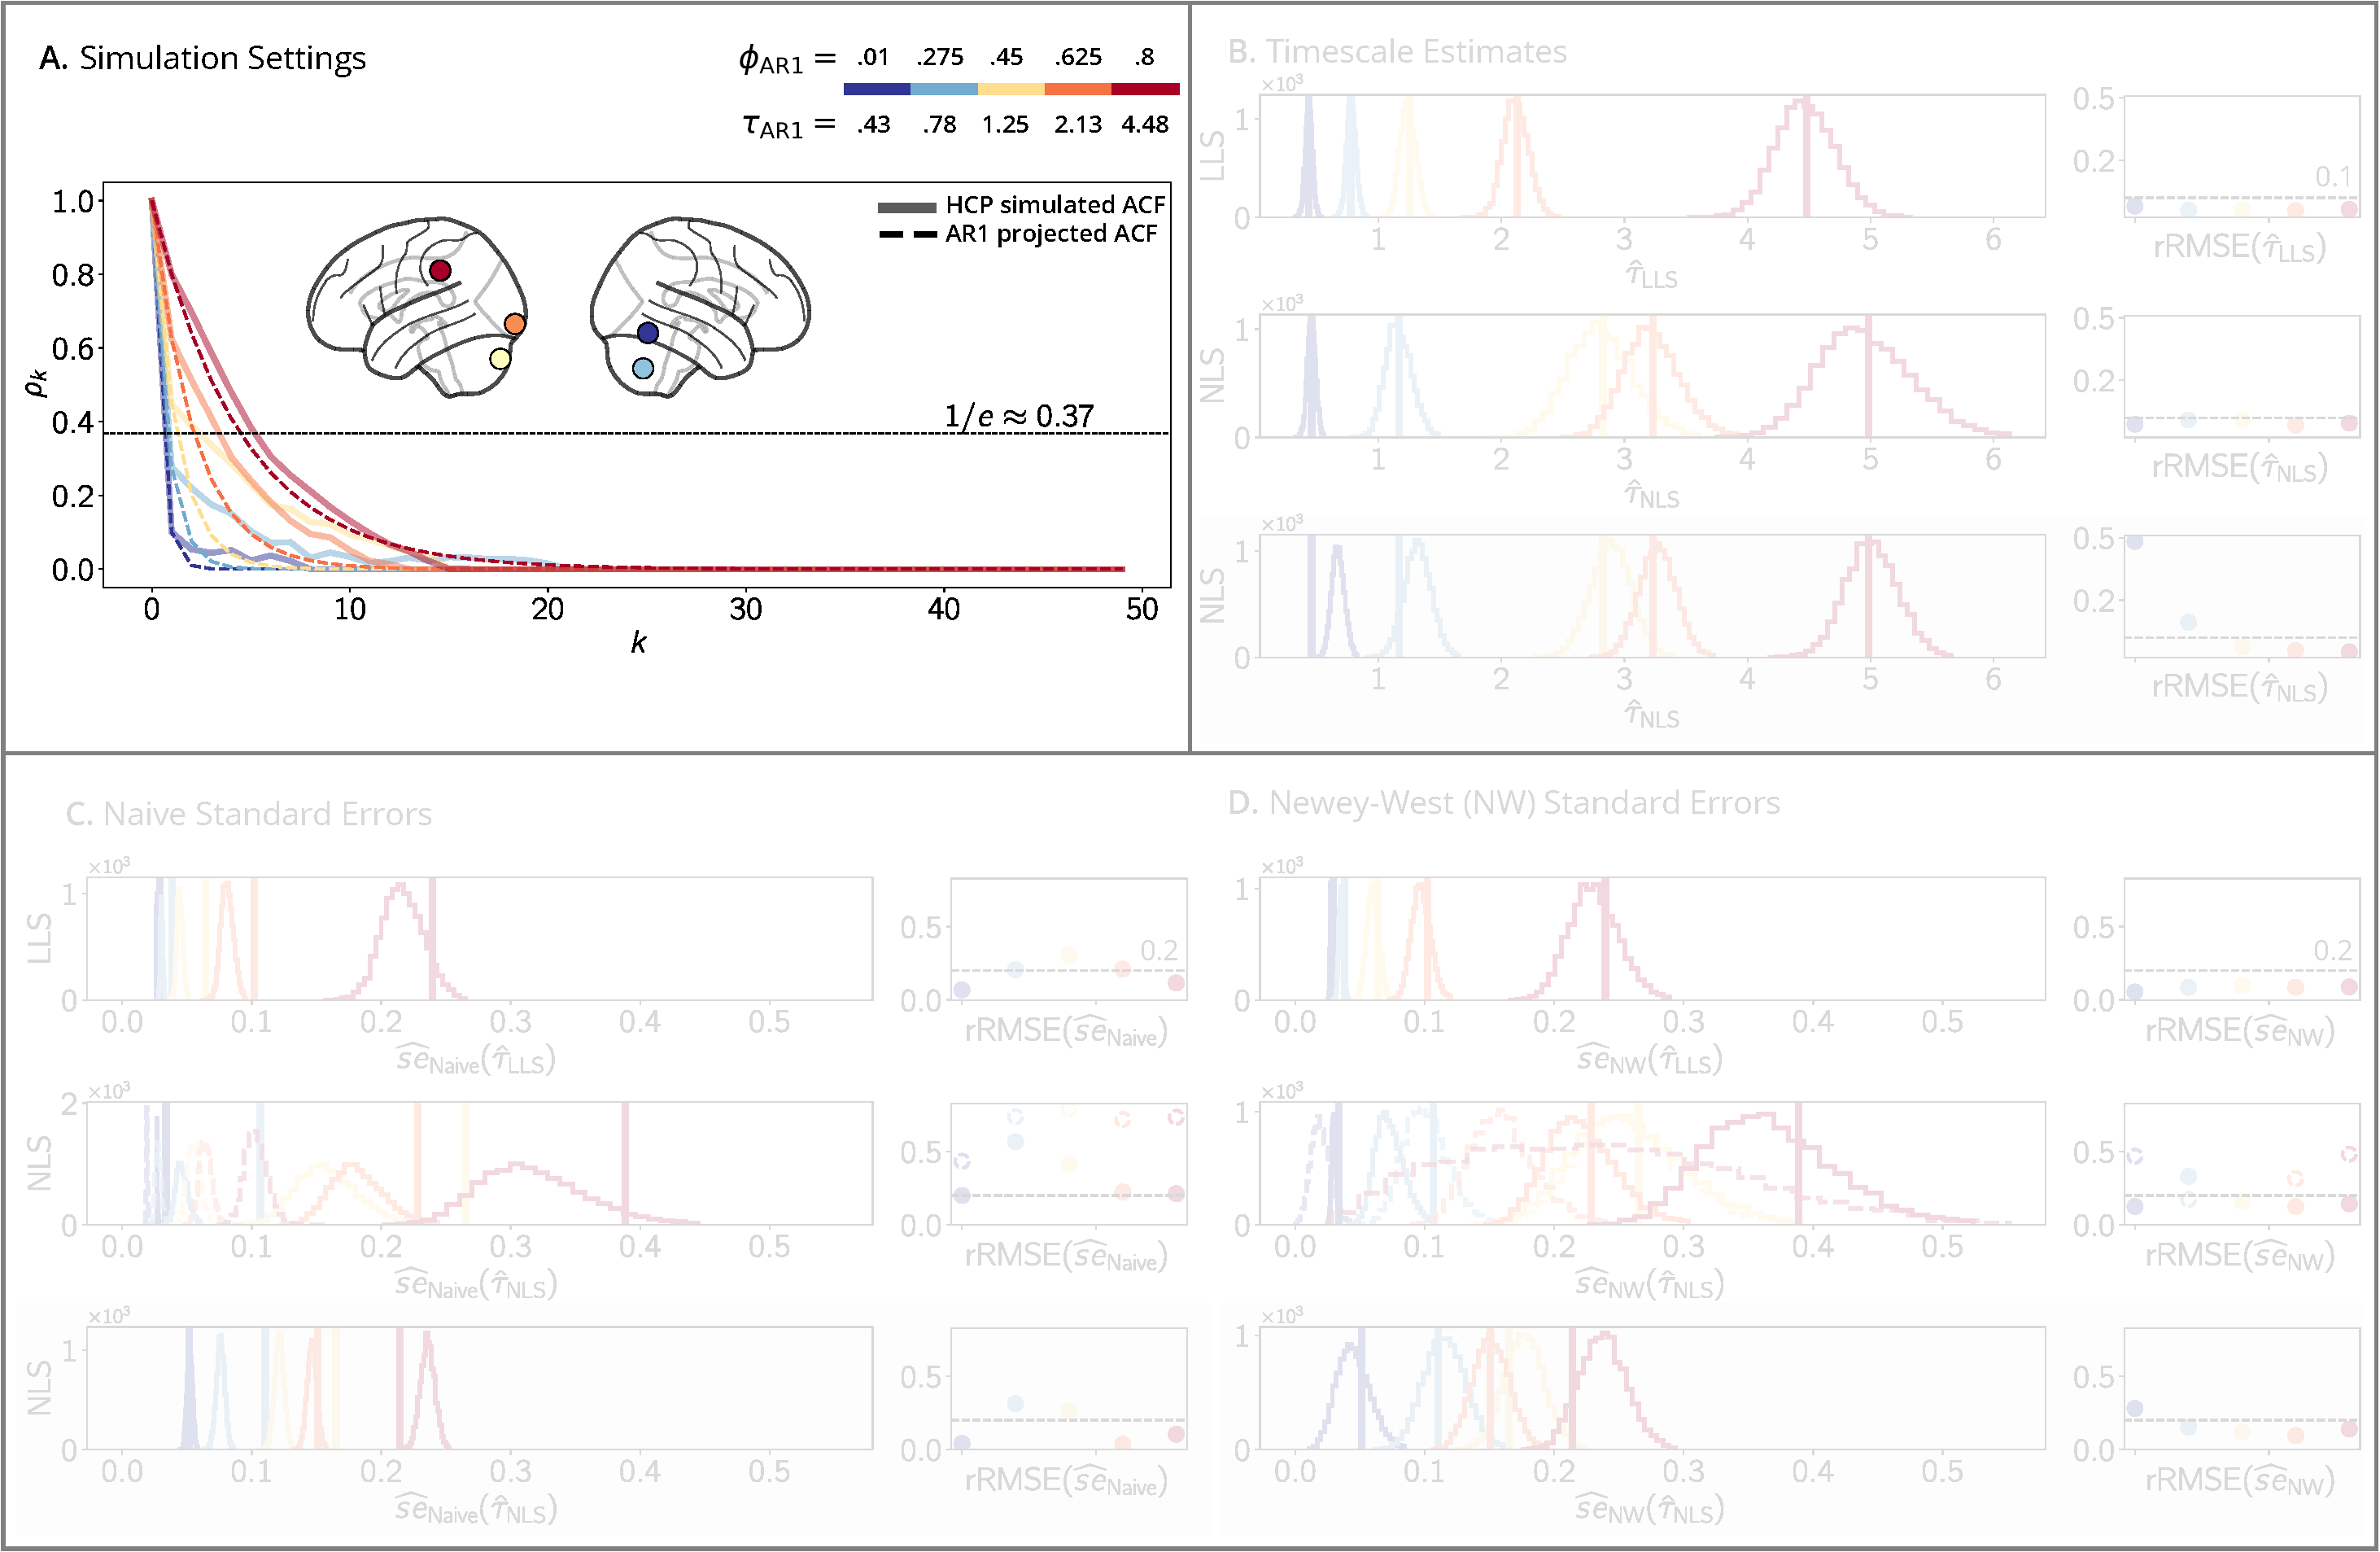
\includegraphics[width=0.85\textwidth]{docs/wnar/hcp-results-1.pdf}}
\only<2>{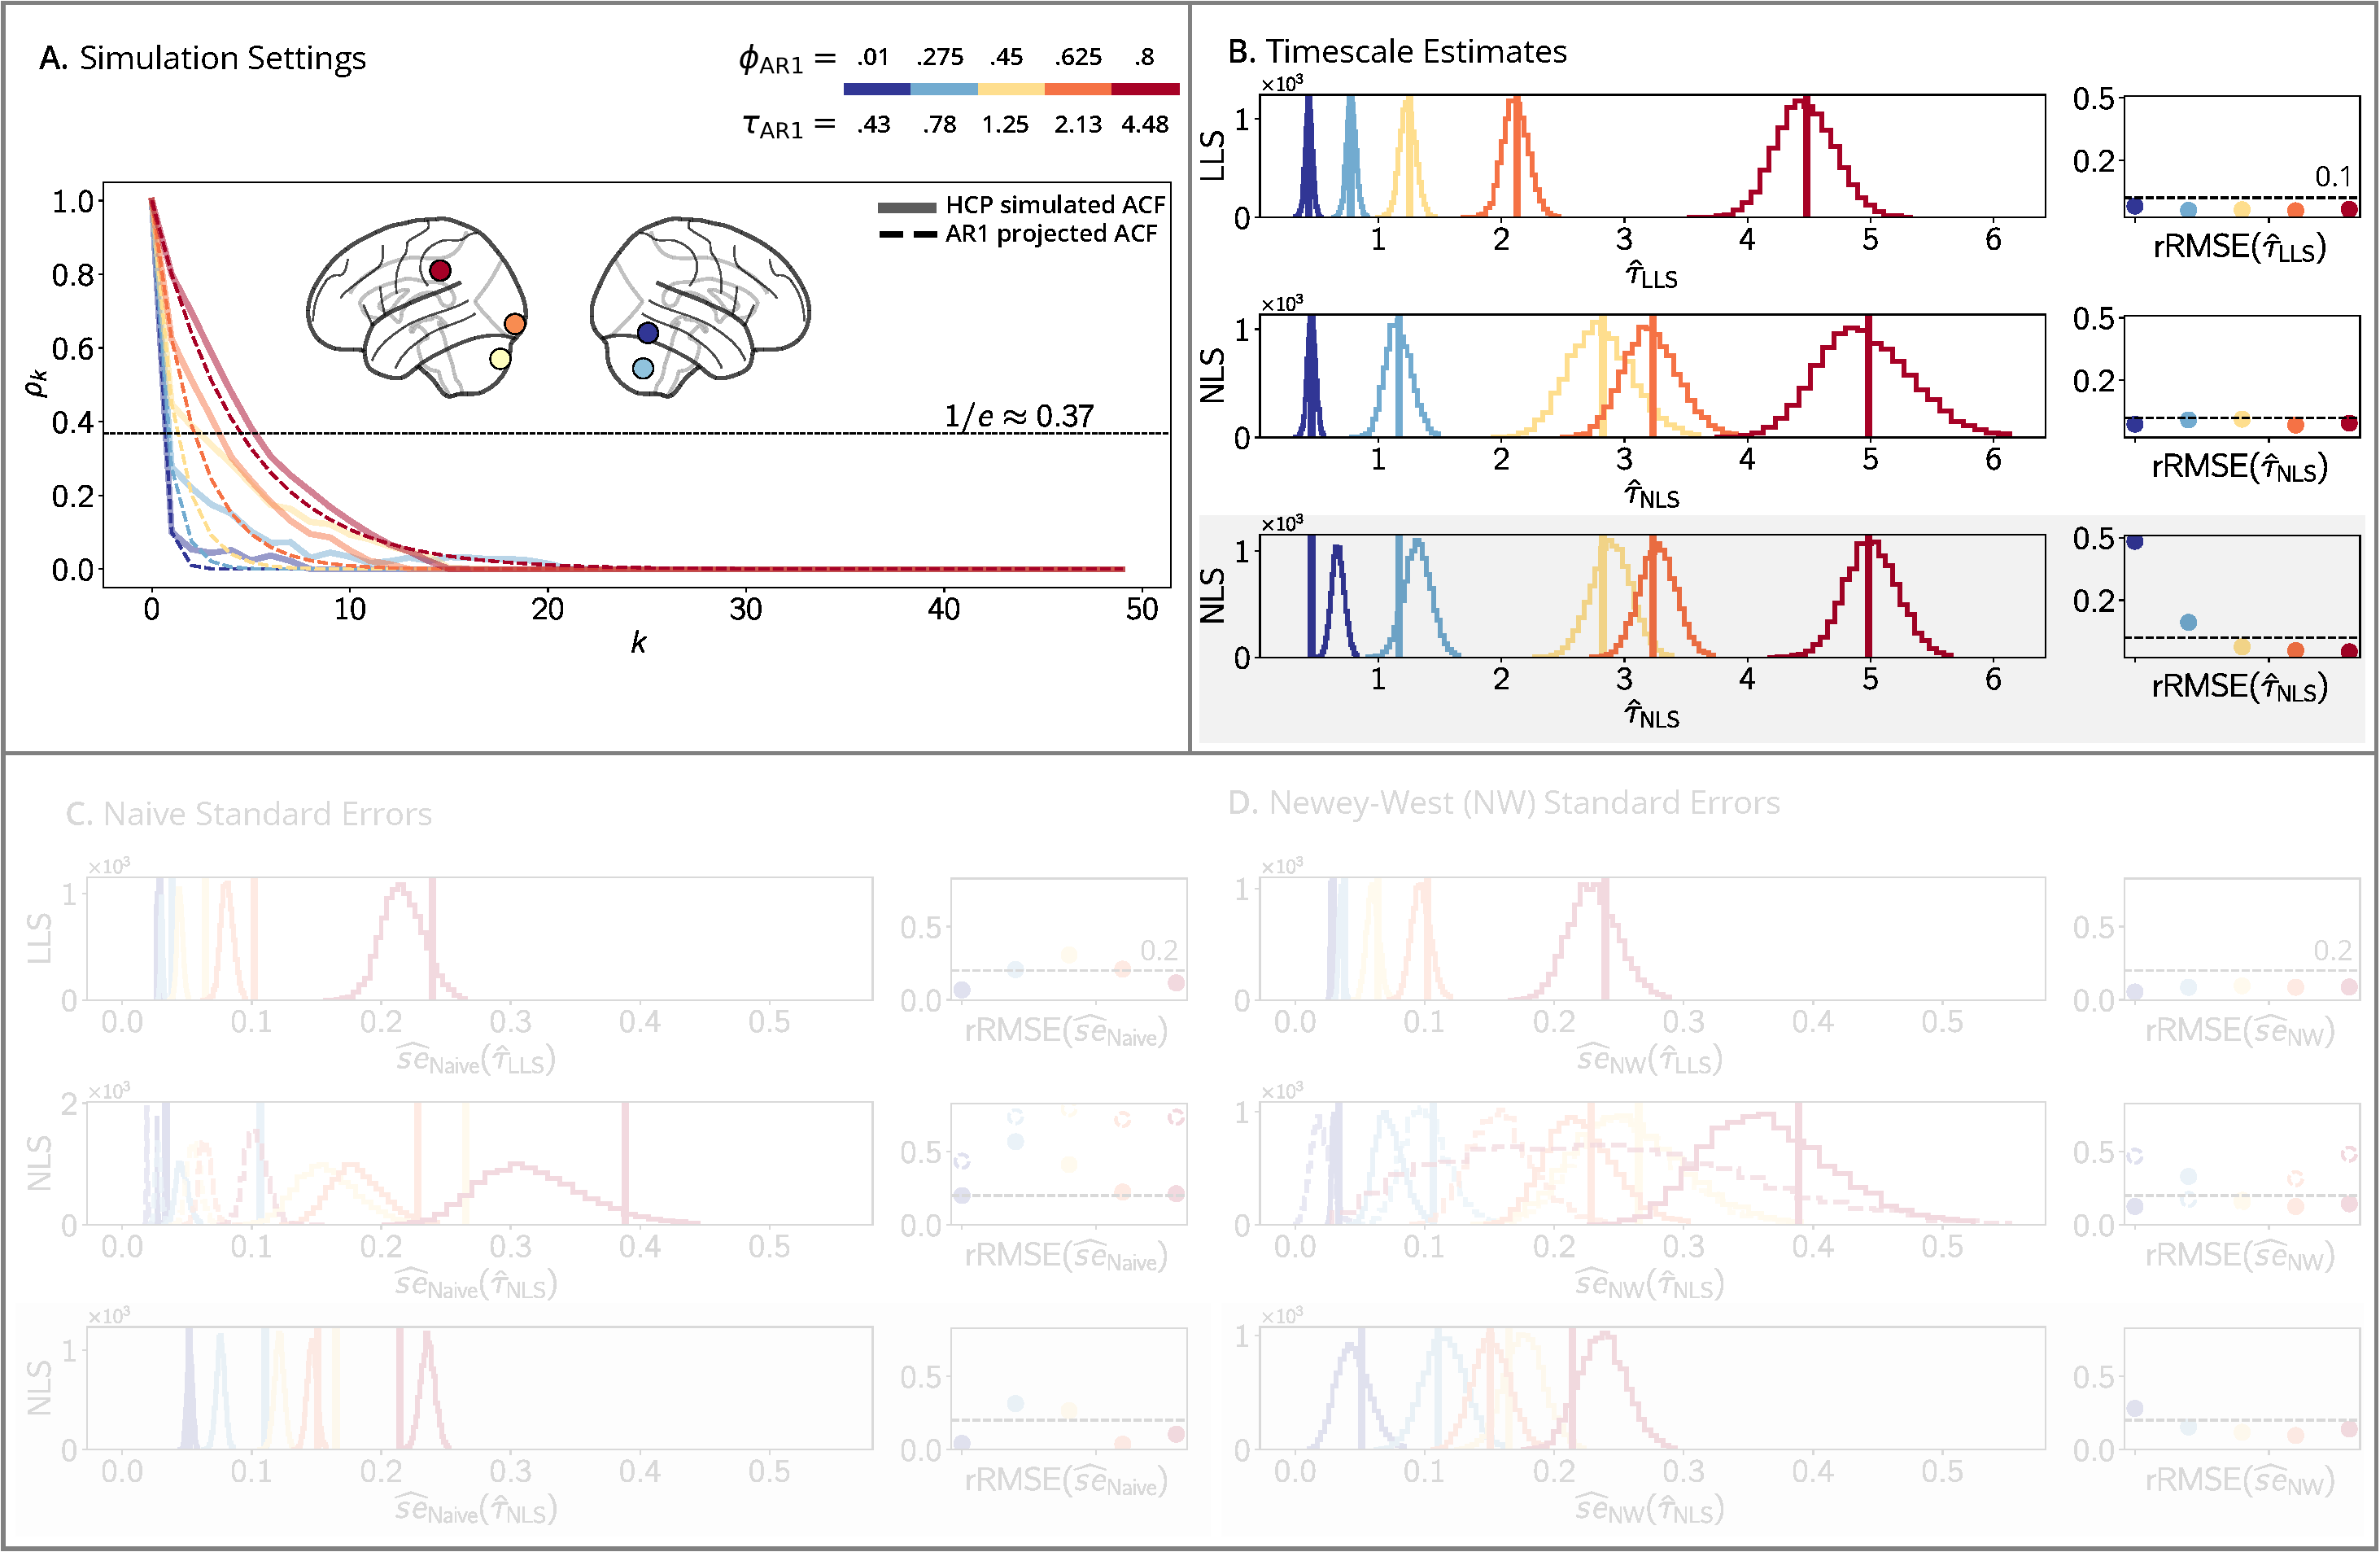
\includegraphics[width=0.85\textwidth]{docs/wnar/hcp-results-2.pdf}}
\only<3>{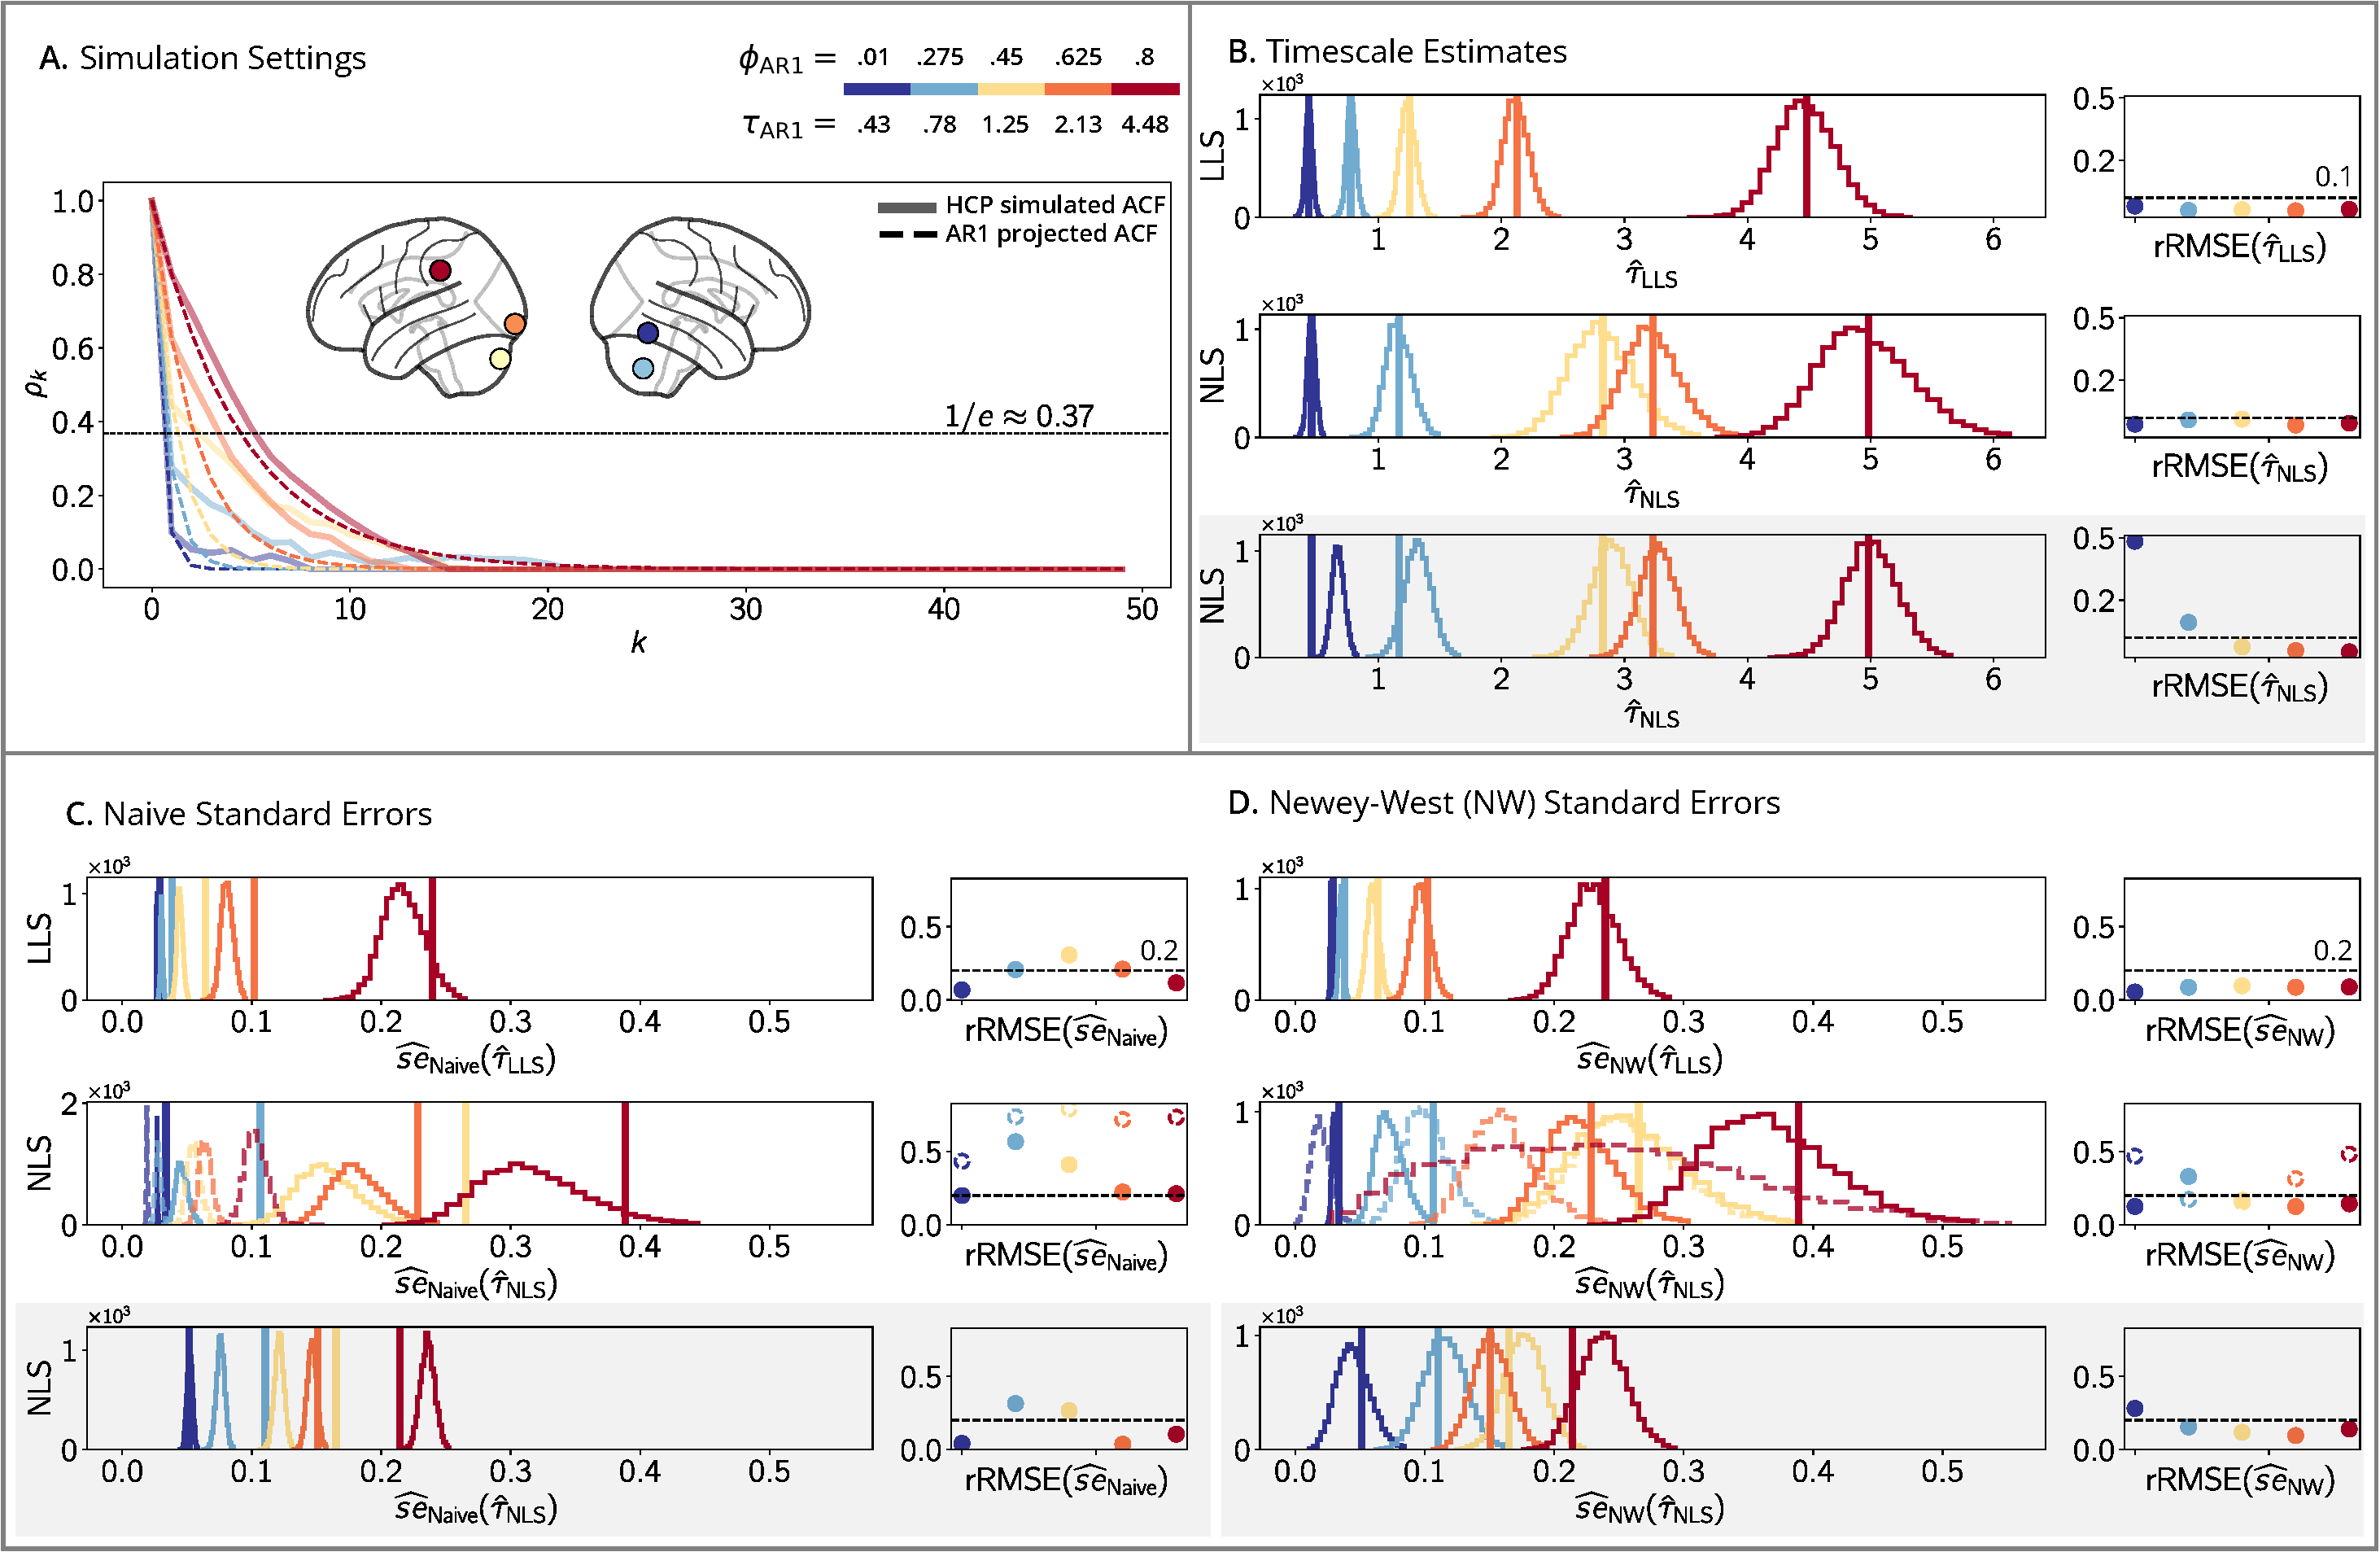
\includegraphics[width=0.85\textwidth]{docs/wnar/hcp-results-3.pdf}}
\end{frame}

% section %
\section{4. Data Analysis}


% slide %
\begin{frame}{Subject-Level Results}
$N = 1$ subject, \;$T = 4,800$ timepoints,\; $V = 64,984$ vertices \hfill Human Connectome Project (HCP)
\vfill
\centering
\includegraphics[width=0.9\textwidth]{docs/wnar/hcp1-results.pdf}
\end{frame}

% slide %
\begin{frame}{Group-Level Results}
$N = 180$ subjects, \;$T = 4,800$ timepoints,\; $V = 64,984$ vertices \hfill  Human Connectome Project (HCP)
\vfill
\centering
\includegraphics[width=0.9\textwidth]{docs/wnar/hcp180-results.pdf}
\end{frame}

% section %
\section{5. Conclusions}

% slide %
\begin{frame}{Conclusions}
\begin{enumerate}
    \item We formalized and compared time- and autocorrelation-domain methods for fMRI timescale mapping.
    \vspace{2mm}
    \item These methods are consistent under broad conditions (stationary, mixing) but estimate different timescale values.
    \vspace{2mm}
    \item In addition, we show that robust standard errors enable valid inference, addressing a key limitation of prior work.
    \vspace{2mm}
    \item Comparatively, the time-domain method produces more accurate estimates under model misspecification and remains computationally efficient for high-dimensional fMRI data.
    \vspace{2mm}
    \item We demonstrate that both time- and autocorrelation-domain methods yield maps aligned with known functional brain organization.
    \vspace{2mm}
    \item Our methods can provide a foundation for future research on the role of timescales in brain structure and function.
\end{enumerate}
\end{frame}

% section/slide %
\begin{frame}{References}
\bibliography{docs/zotero}

\vspace{5mm}
\centering{\Large Thank you!}
\vspace{1cm}

\begin{columns}
\column{0.5\textwidth}
\centering
\textbf{paper}:\\

\includegraphics[width=0.35\textwidth]{docs/wnar/paper.png}\\
https://doi.org/10.1101/2025.04.23.650300
\column{0.5\textwidth}
\centering
\textbf{code}:\\

\includegraphics[width=0.35\textwidth]{docs/wnar/code.png}\\
https://github.com/griegner/fmri-timescales
\end{columns}
\end{frame}
\end{document}